\documentclass{article}
\usepackage{geometry}
\usepackage{graphicx}
\usepackage{float}
\usepackage{titlesec}
\geometry{a4paper, left=2cm, right=2cm, top=2cm, bottom=2cm}
\titleformat{\section}{\normalfont\fontsize{14}{15}\bfseries}{\thesection}{1em}{}
\usepackage{hyperref}
\usepackage{ctex}
\usepackage{caption}
\usepackage{subcaption}
\usepackage{listings}
\usepackage{xcolor}

% 设置代码样式
\lstdefinestyle{Style}{
    language=bash, % 设置代码语言
    basicstyle=\ttfamily\small, % 设置字体样式和大小
    keywordstyle=\color{blue}, % 关键字颜色
    commentstyle=\color{green!40!black}, % 注释颜色
    stringstyle=\color{purple}, % 字符串颜色
    numbers=left, % 行号显示在左侧
    numberstyle=\tiny\color{gray}, % 行号样式
    stepnumber=1, % 行号逐行显示
    numbersep=8pt, % 行号与代码的距离
    showspaces=false, % 是否显示空格
    showstringspaces=false, % 是否显示字符串中的空格
    showtabs=false, % 是否显示制表符
    tabsize=4, % 制表符的大小
    frame=single, % 边框类型,可以是 single, lines, none, ...
    frameround=tttt, % 边框角落样式,可以是 tttt, trbl, none, ...
    backgroundcolor=\color{white}, % 背景颜色
    breaklines=true, % 自动断行
    breakatwhitespace=true, % 在空格处断行
    captionpos=b, % 代码块标题位置(b 表示底部)
    extendedchars=true, % 支持特殊字符
    morekeywords={val, var, def, import}, % 添加额外的关键字
    inputencoding=utf8, % 输入编码,适用于包含非 ASCII 字符的代码
}

\begin{document}
\title{Data Ingestion Tools实验}
\author{211250109 赵政杰}
\date{\today}
\maketitle
本次实验在实验二所创建的云实例上进行。
\section{任务1:使用Apache Kafka进行数据流}
\subsection*{1.1 安装Kafka}
在实验2中已经在服务器上完成安装Java.\par
使用\lstinline[style = Style]|wget https://mirrors.aliyun.com/apache/kafka/3.5.1/kafka_2.12-3.5.1.tgz|获取压缩包并解压。
\begin{figure}[H]
    \centering
    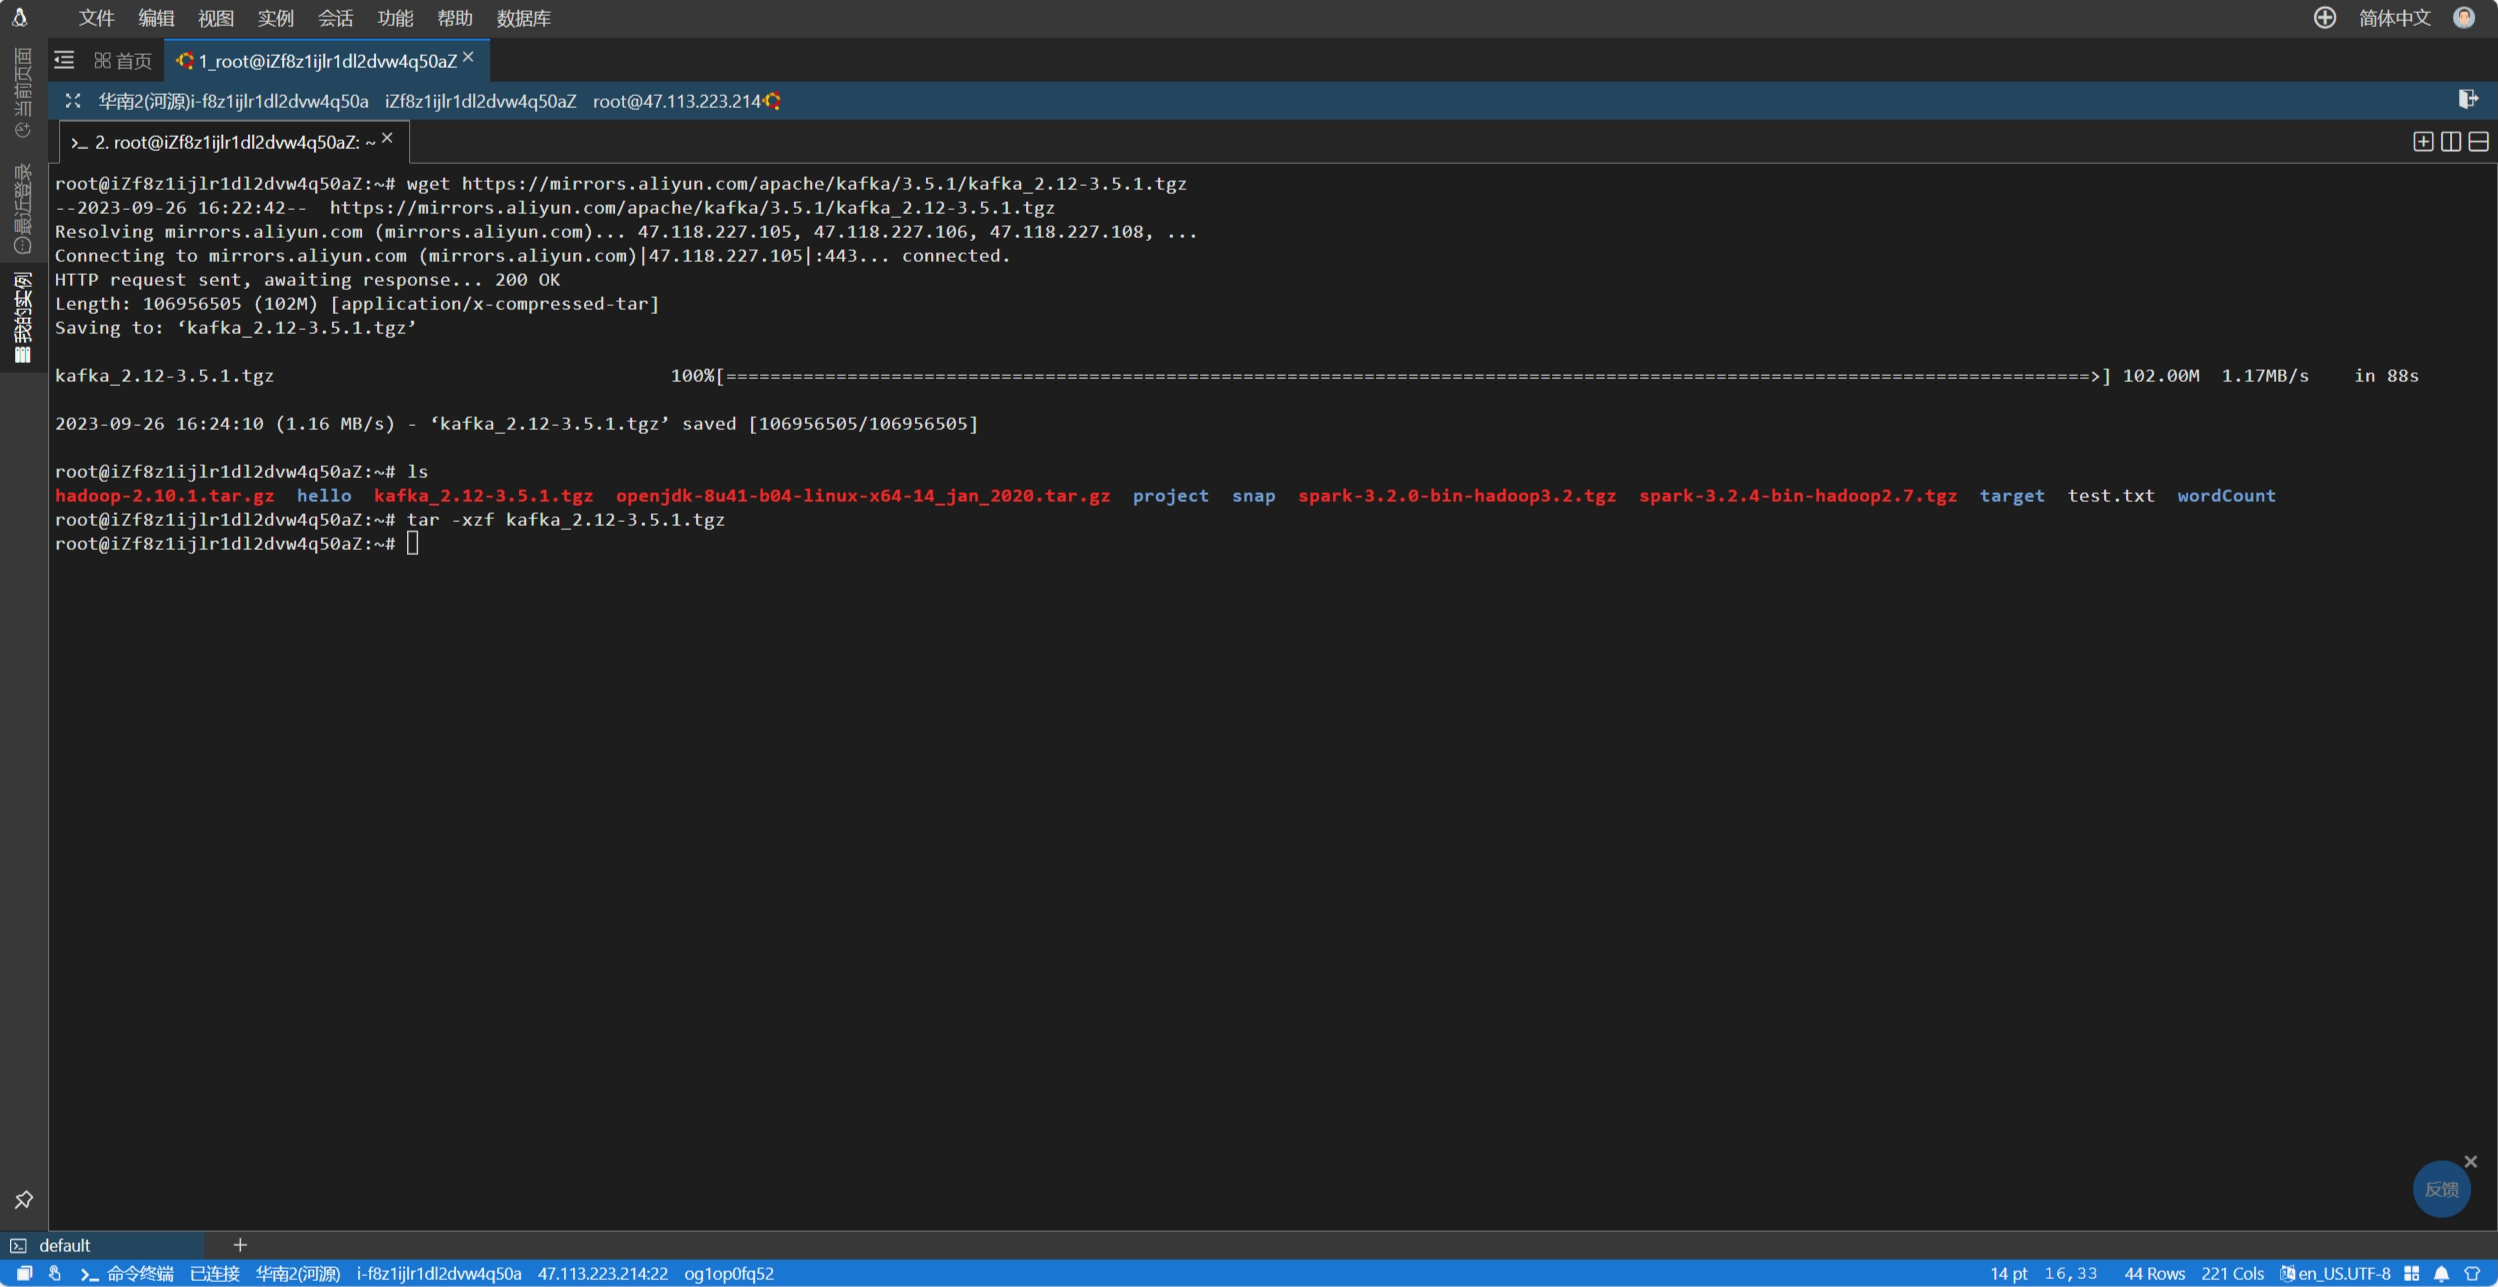
\includegraphics[width=0.7\textwidth]{./pic/2.png}
    \caption{安装Kafka}
\end{figure}
\subsection*{1.2 启动Kafka服务}
\begin{itemize}
    \item 在Kafka目录中,启动Zookeeper服务器。命令为\lstinline[style=Style]|bin/zookeeper-server-start.sh config/zookeeper.properties|
    \begin{figure}[H]
        \centering
        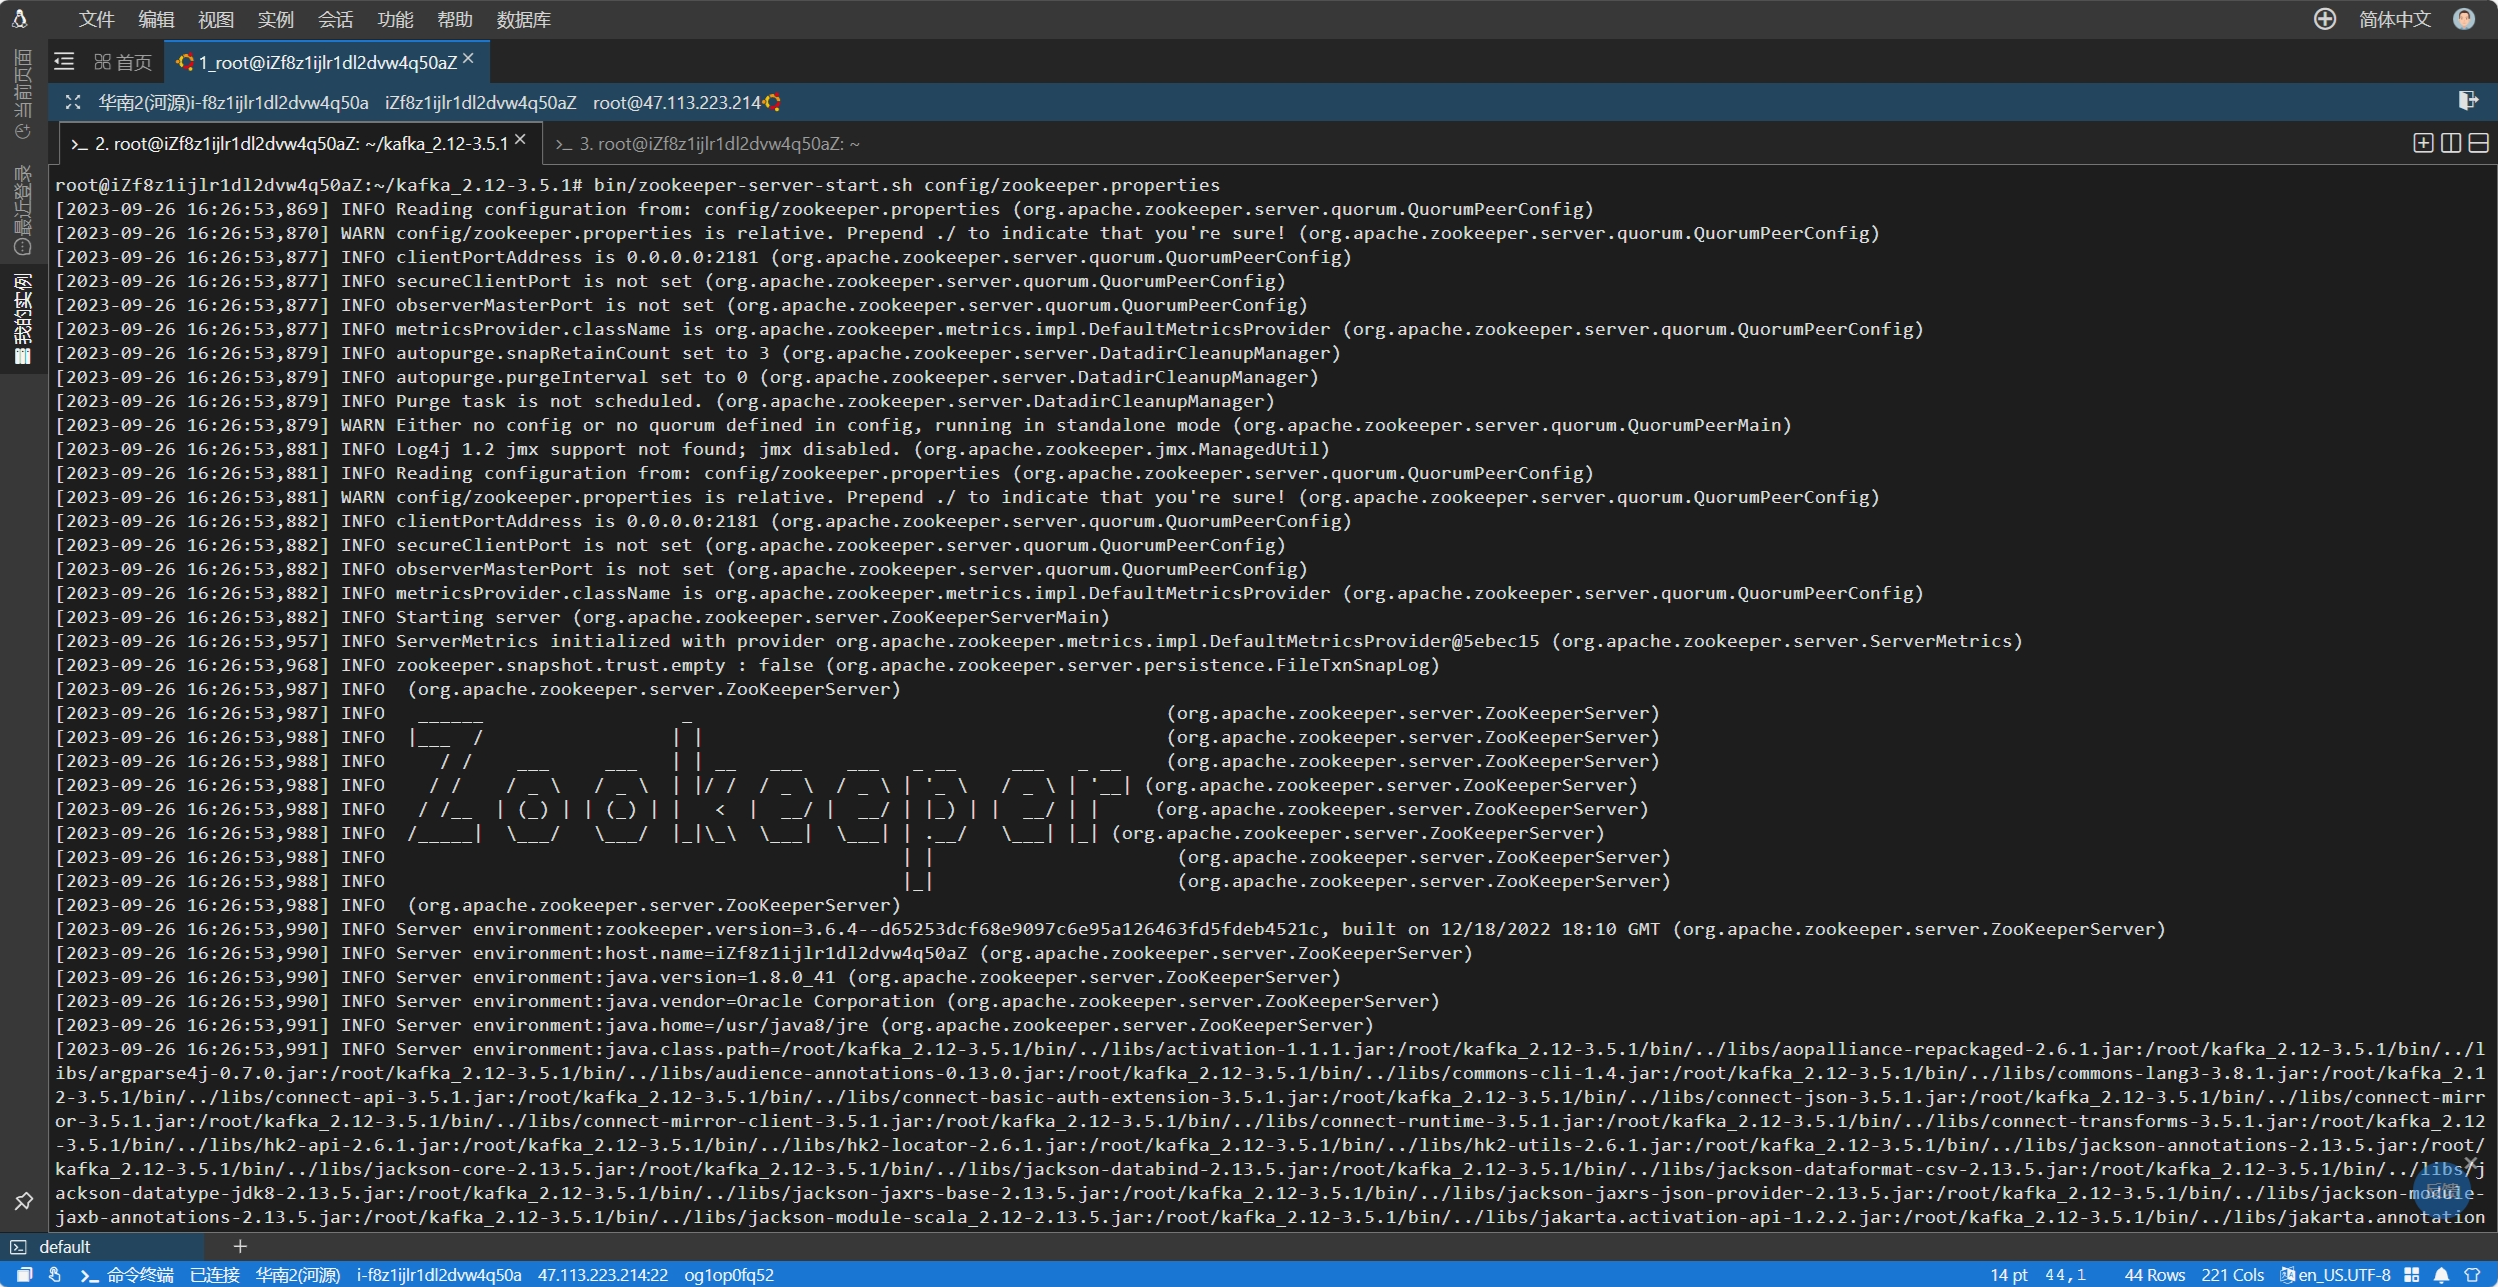
\includegraphics[width=0.7\textwidth]{./pic/3.png}
        \caption{启动Zookeeper}
    \end{figure}
    \item 在新的终端窗口中,启动Kafka服务器。命令为\lstinline[style=Style]|bin/kafka-server-start.sh config/server.properties|
    \begin{figure}[H]
        \centering
        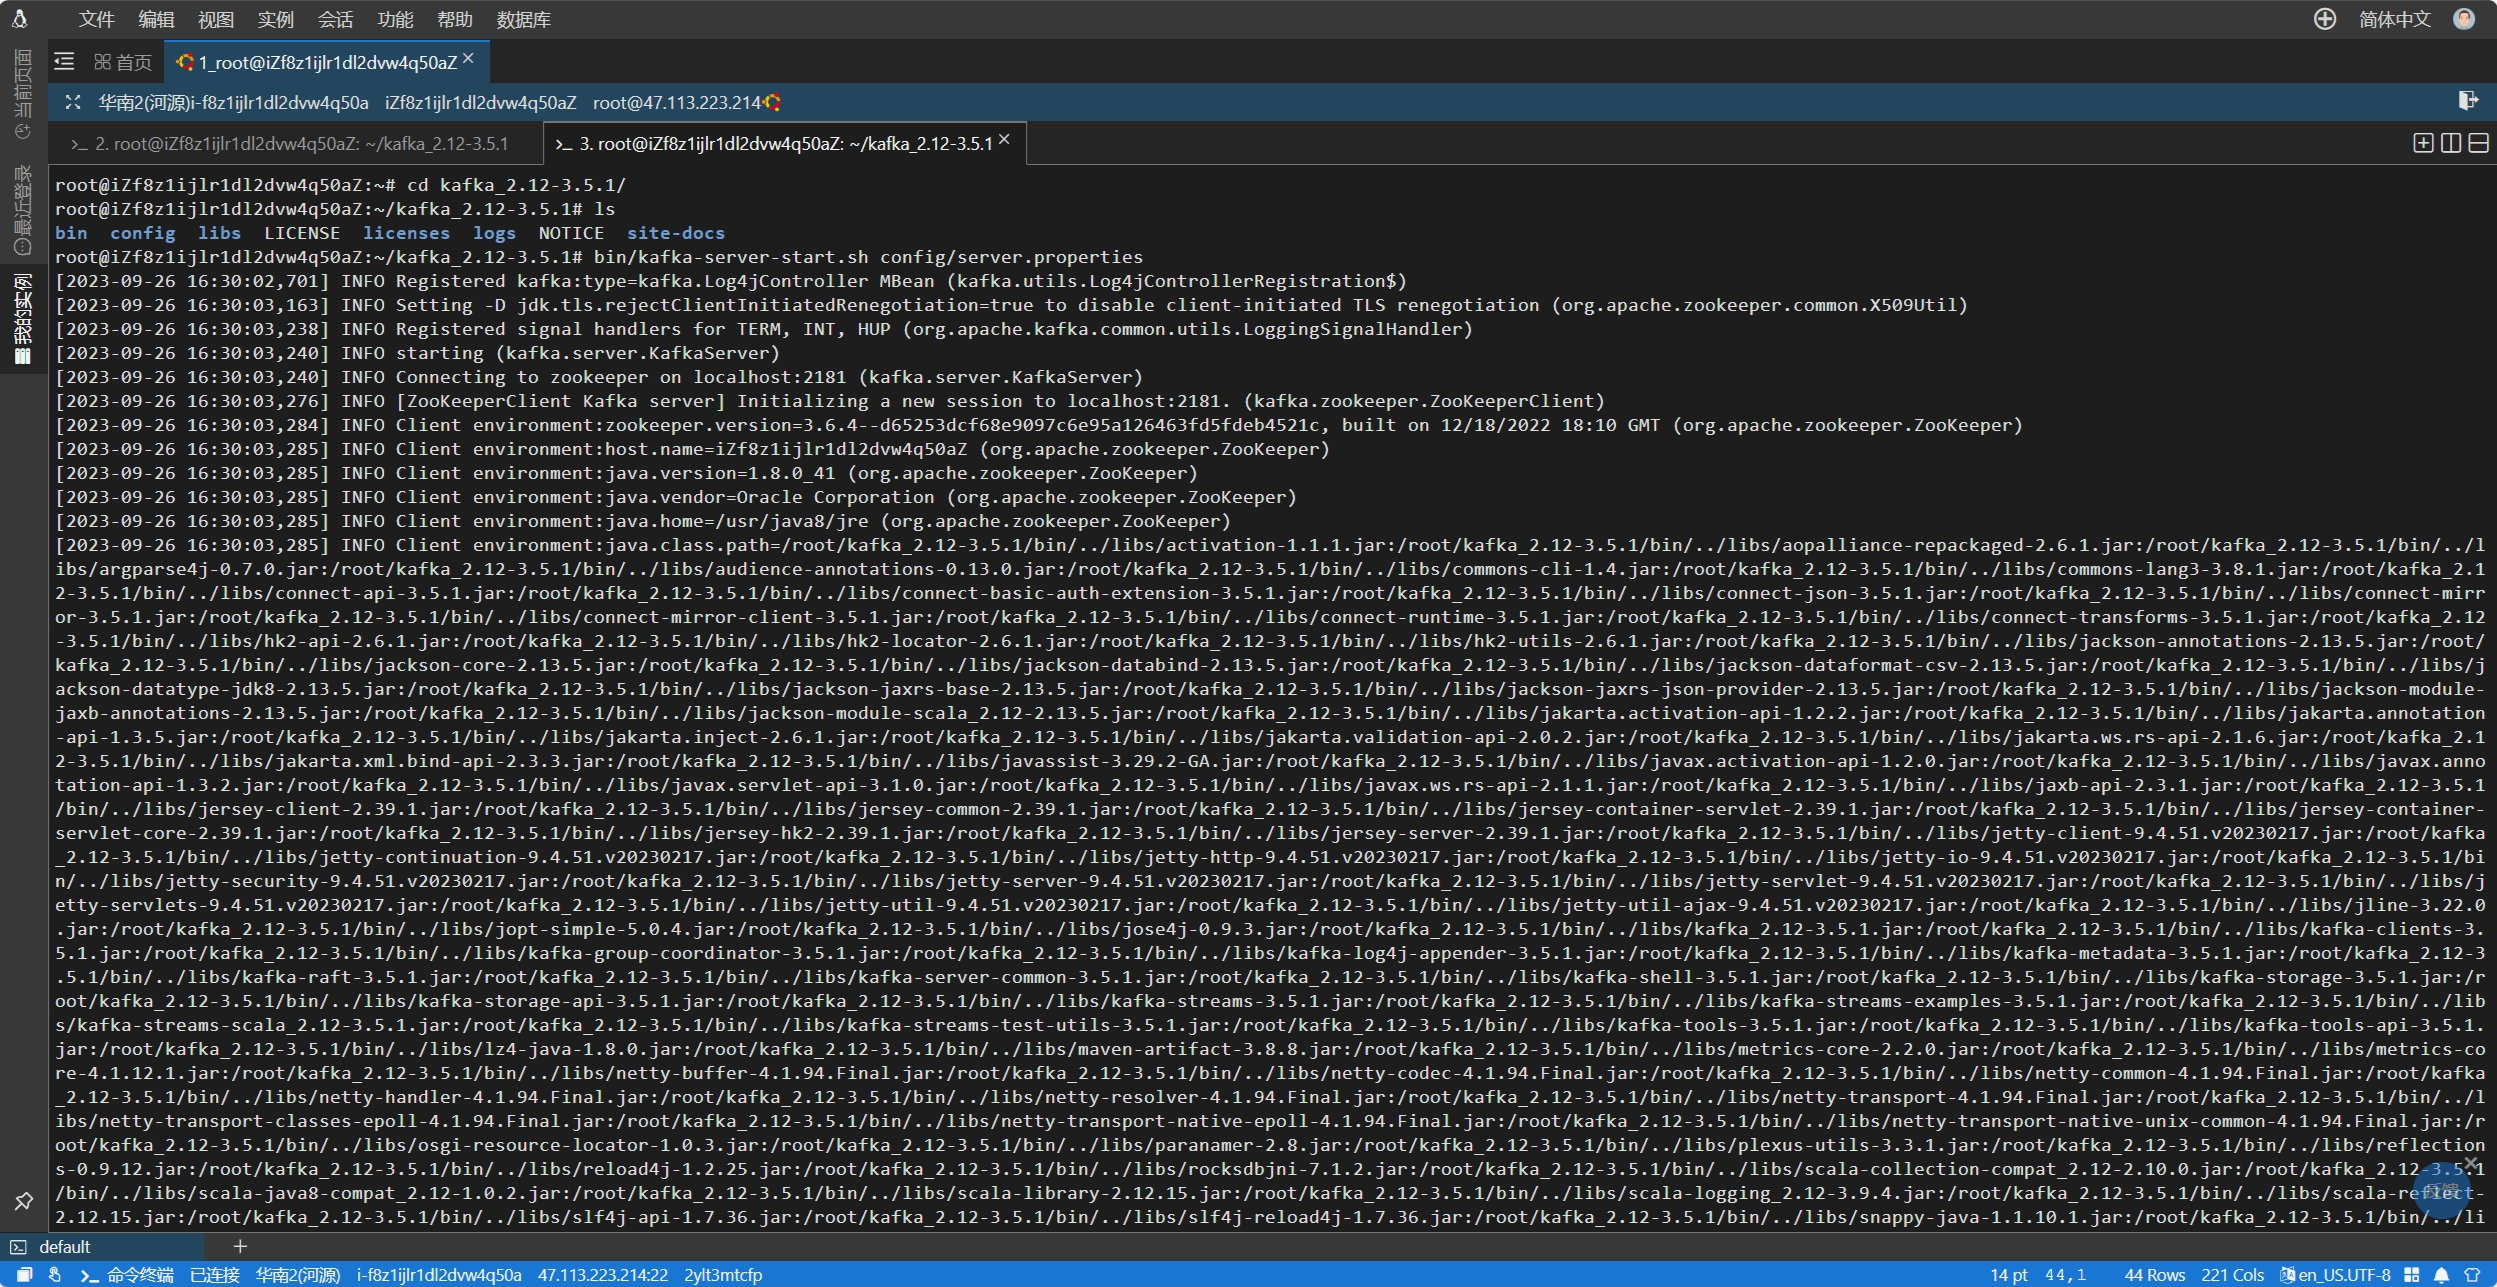
\includegraphics[width=0.7\textwidth]{./pic/4.png}
        \caption{启动Kafka}
    \end{figure}
\end{itemize}
\subsection*{1.3 创建Kafka主题}
使用\lstinline[style = Style]|bin/kafka-topics.sh --create --topic my-topic --bootstrap-server localhost:9092 --partitions 1 --replication-factor 1|
\begin{figure}[H]
    \centering
    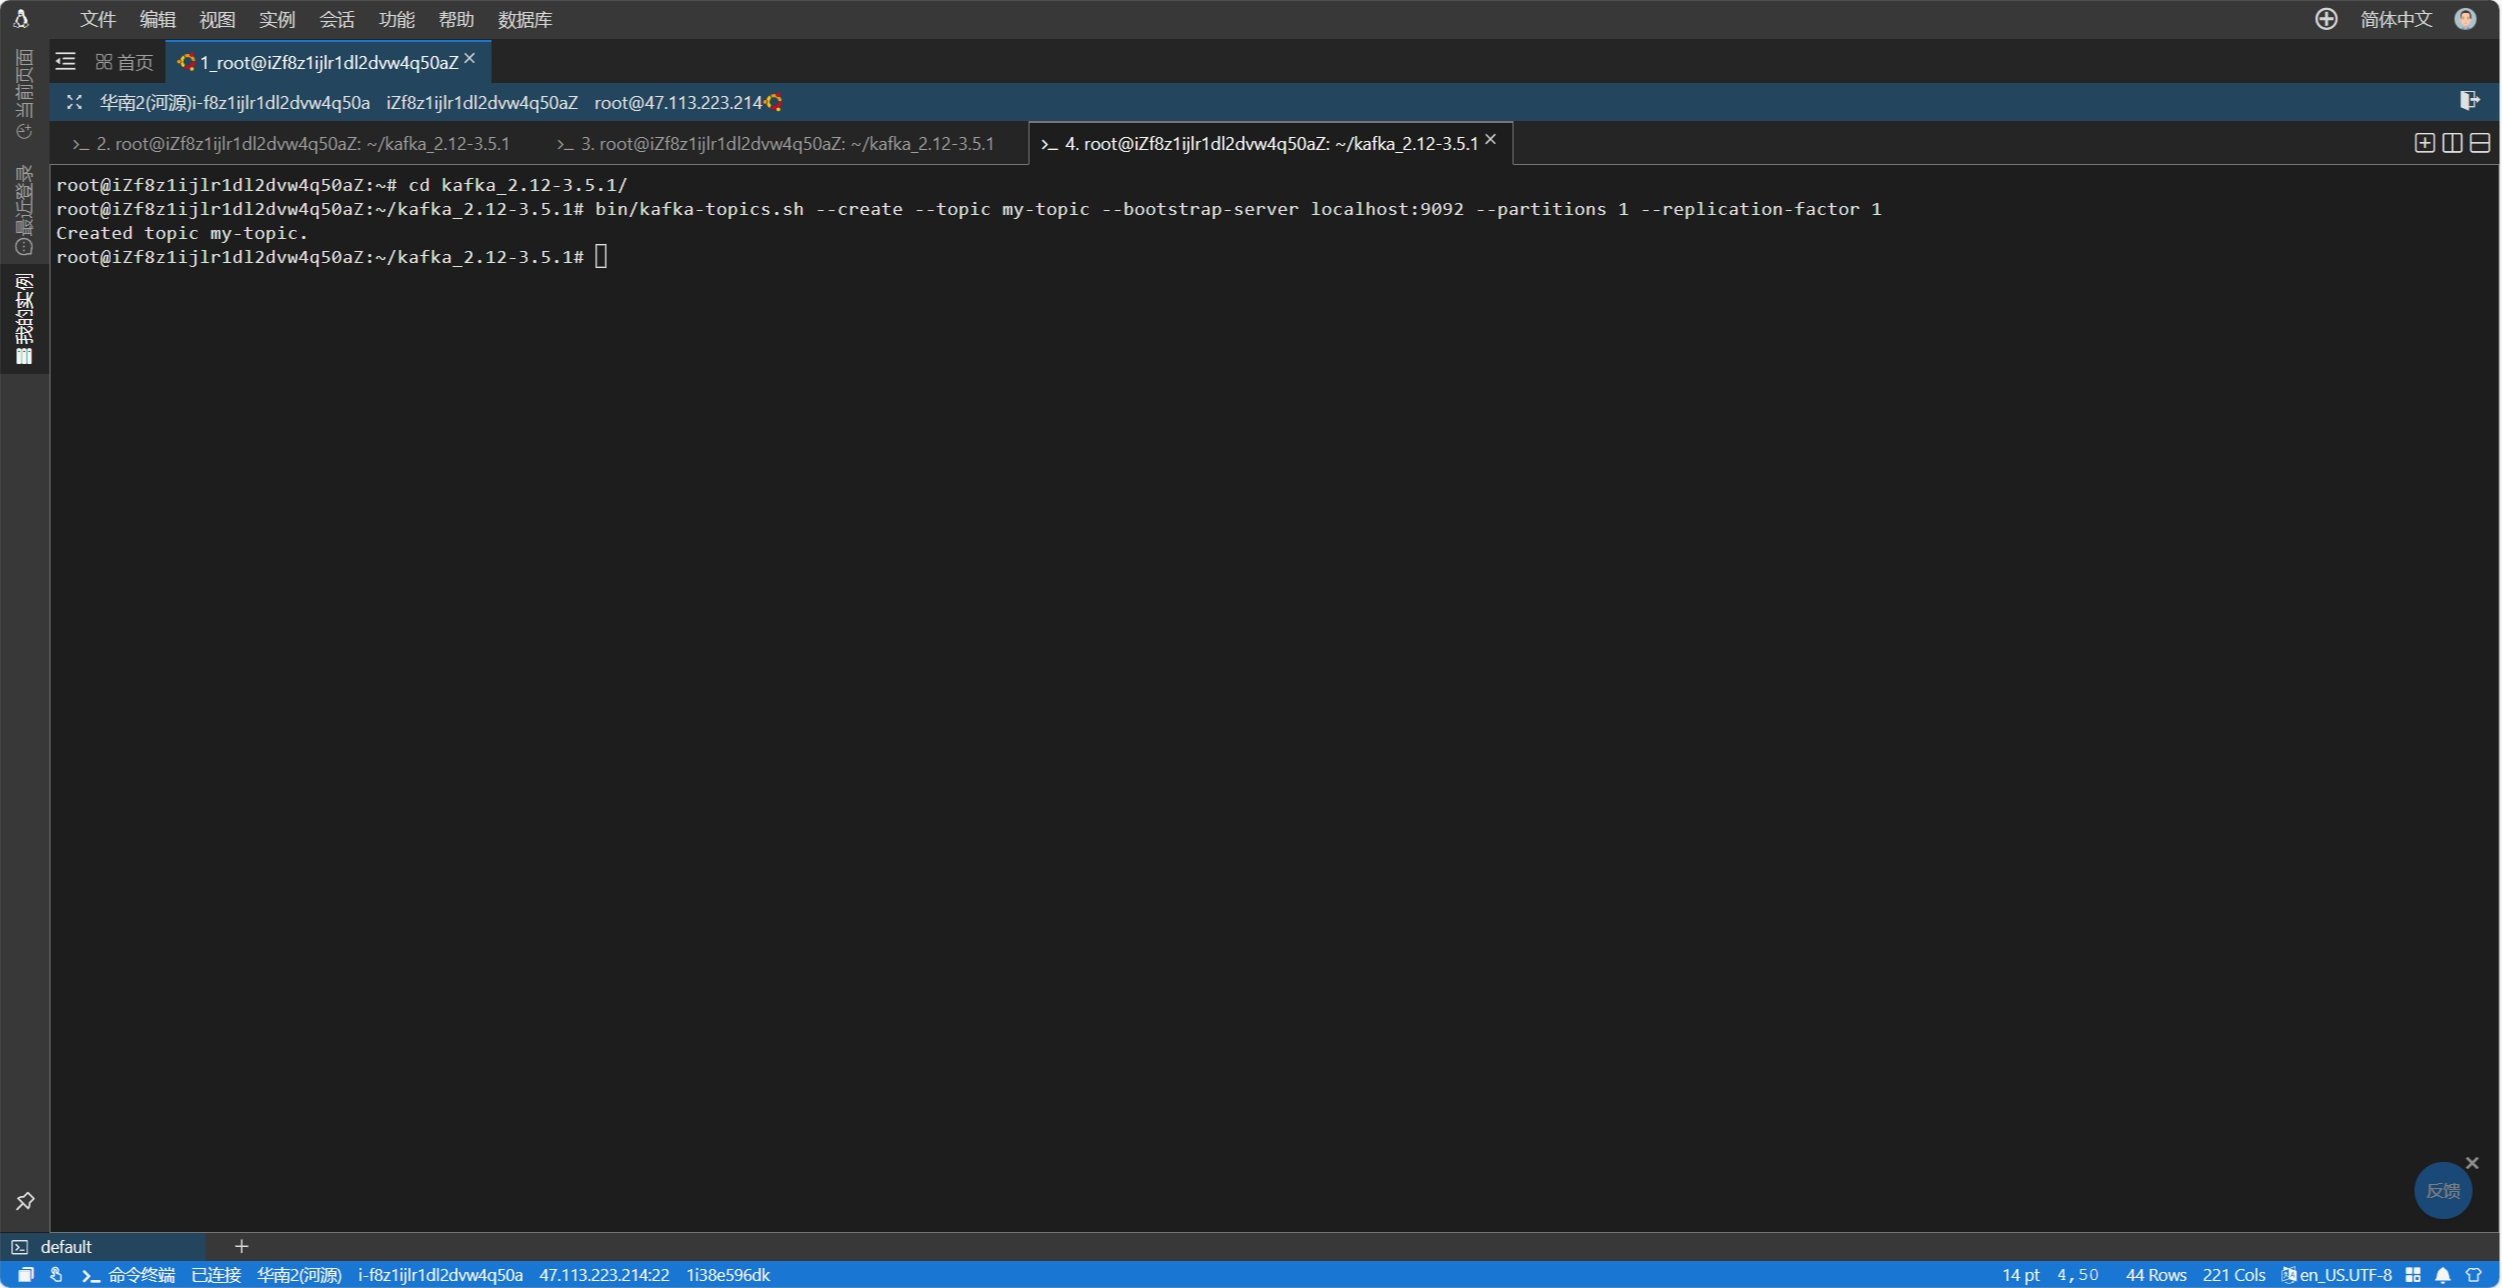
\includegraphics[width=0.7\textwidth]{./pic/5.png}
    \caption{创建my-topic主题}
\end{figure}
\subsection*{1.4 生产和消费消息}
\begin{itemize}
    \item 使用\lstinline[style=Style]|bin/kafka-console-producer.sh --topic my-topic --bootstrap-server localhost:9092|创建生产者。
    \begin{figure}[H]
        \centering
        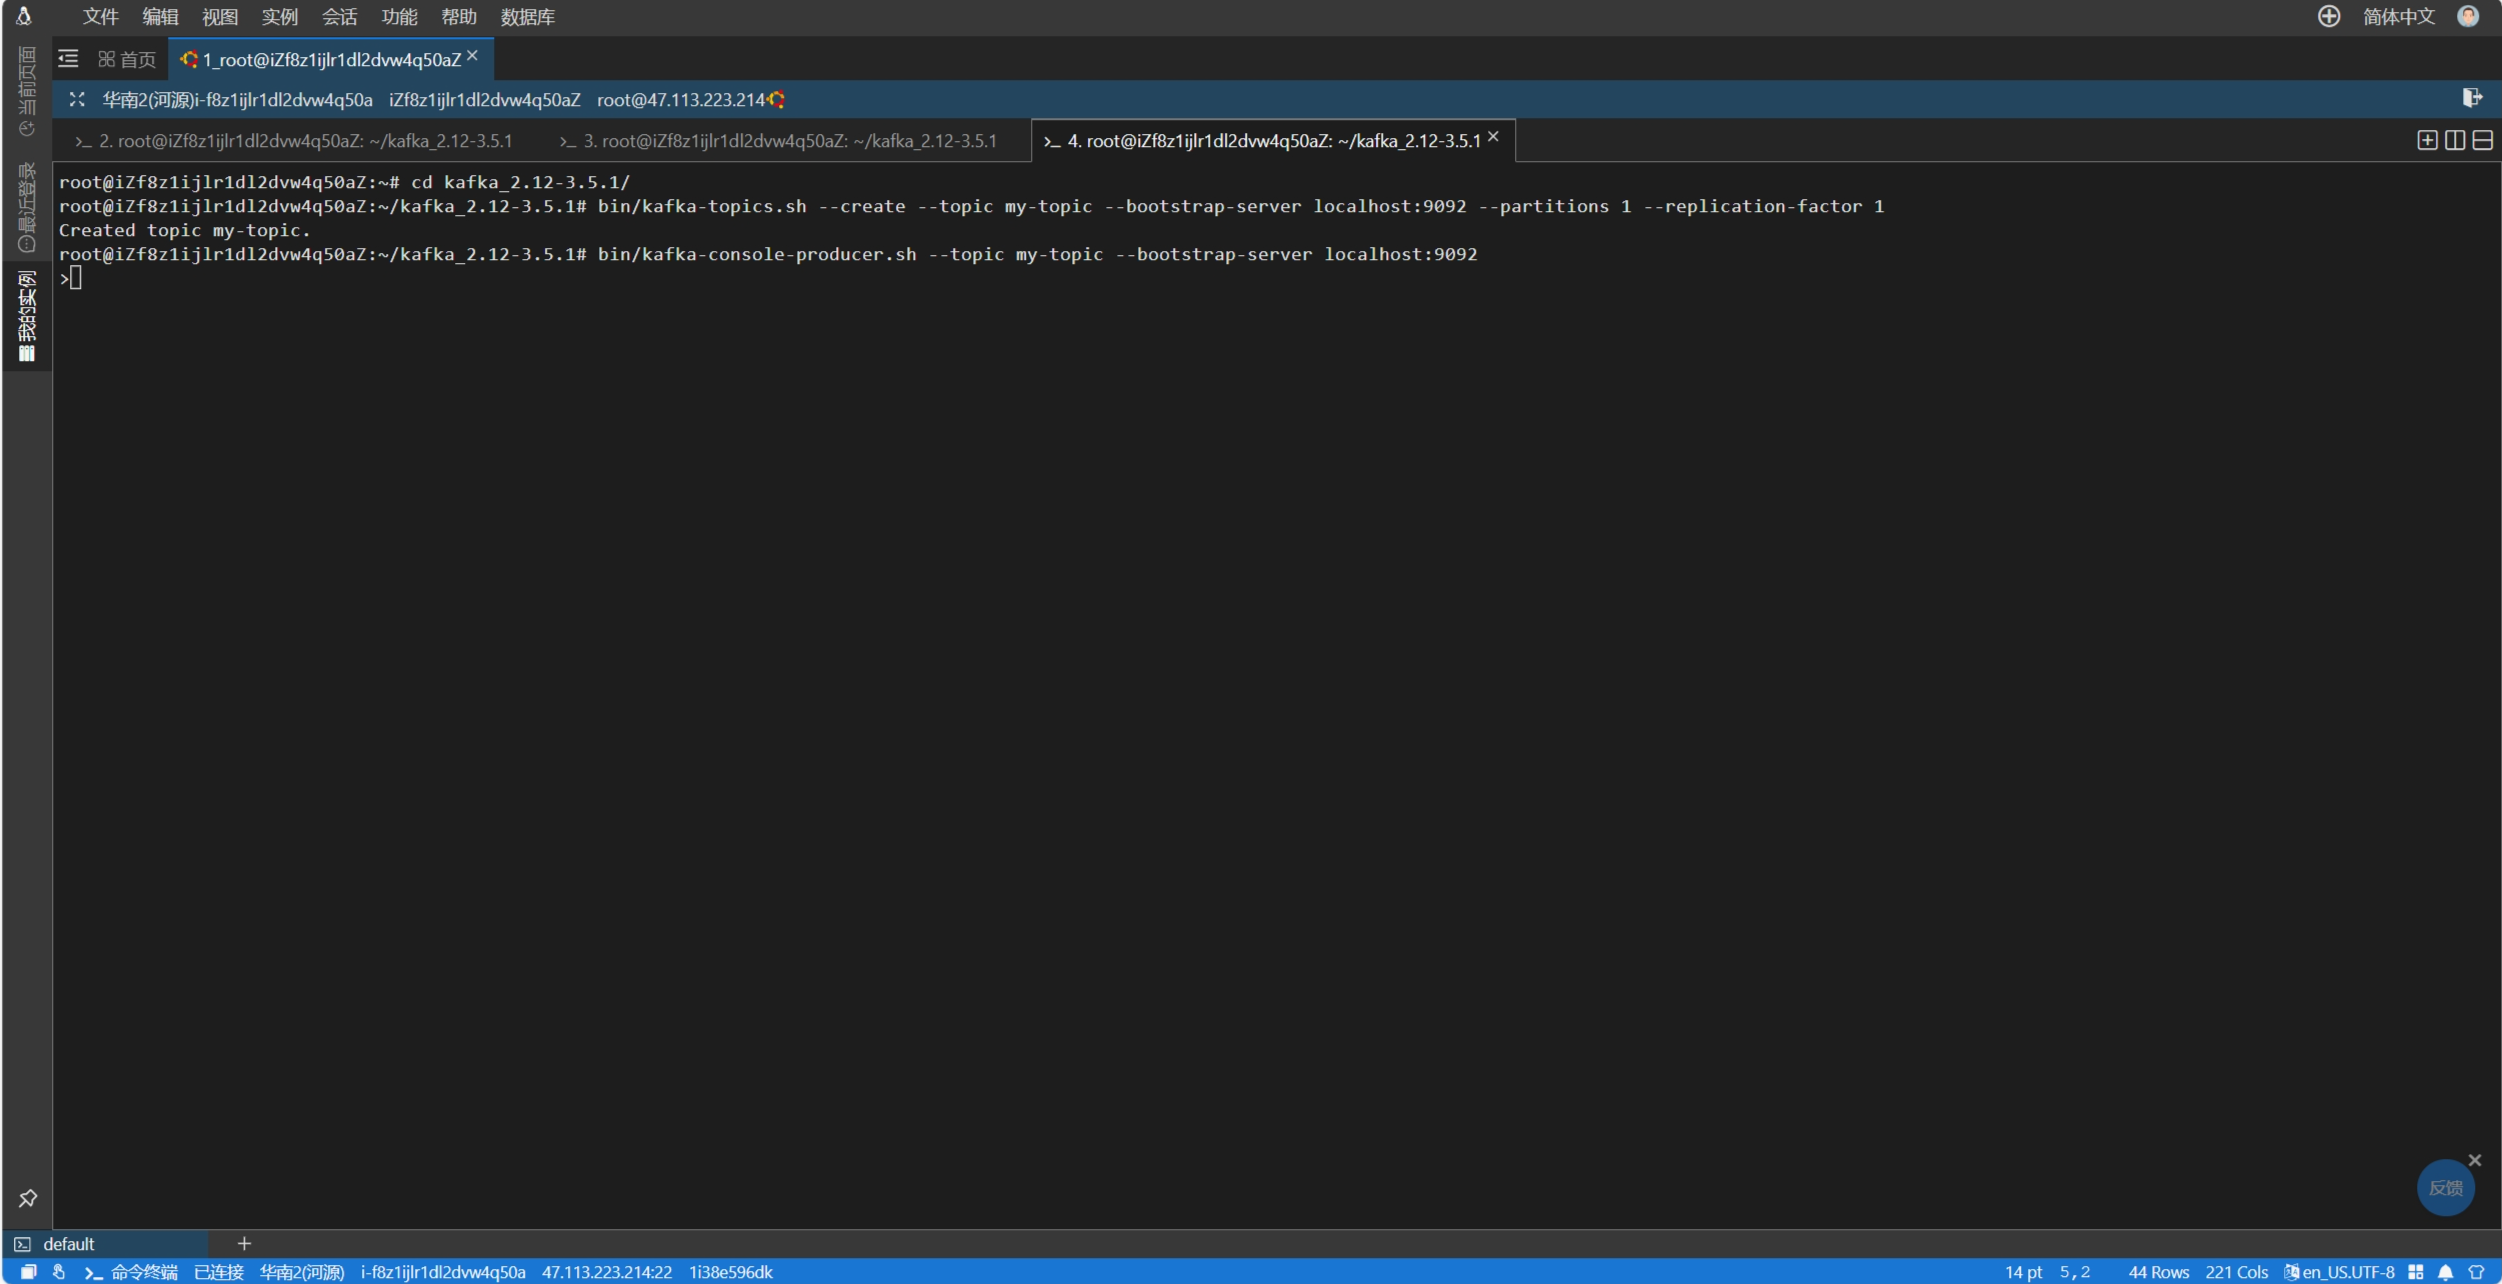
\includegraphics[width=0.5\textwidth]{./pic/6.png}
        \caption{创建生产者}
    \end{figure}
    \item 使用\lstinline[style=Style]|bin/kafka-console-consumer.sh --topic my-topic --bootstrap-server localhost:9092 --from-beginning|创建消费者。
    \begin{figure}[H]
        \centering
        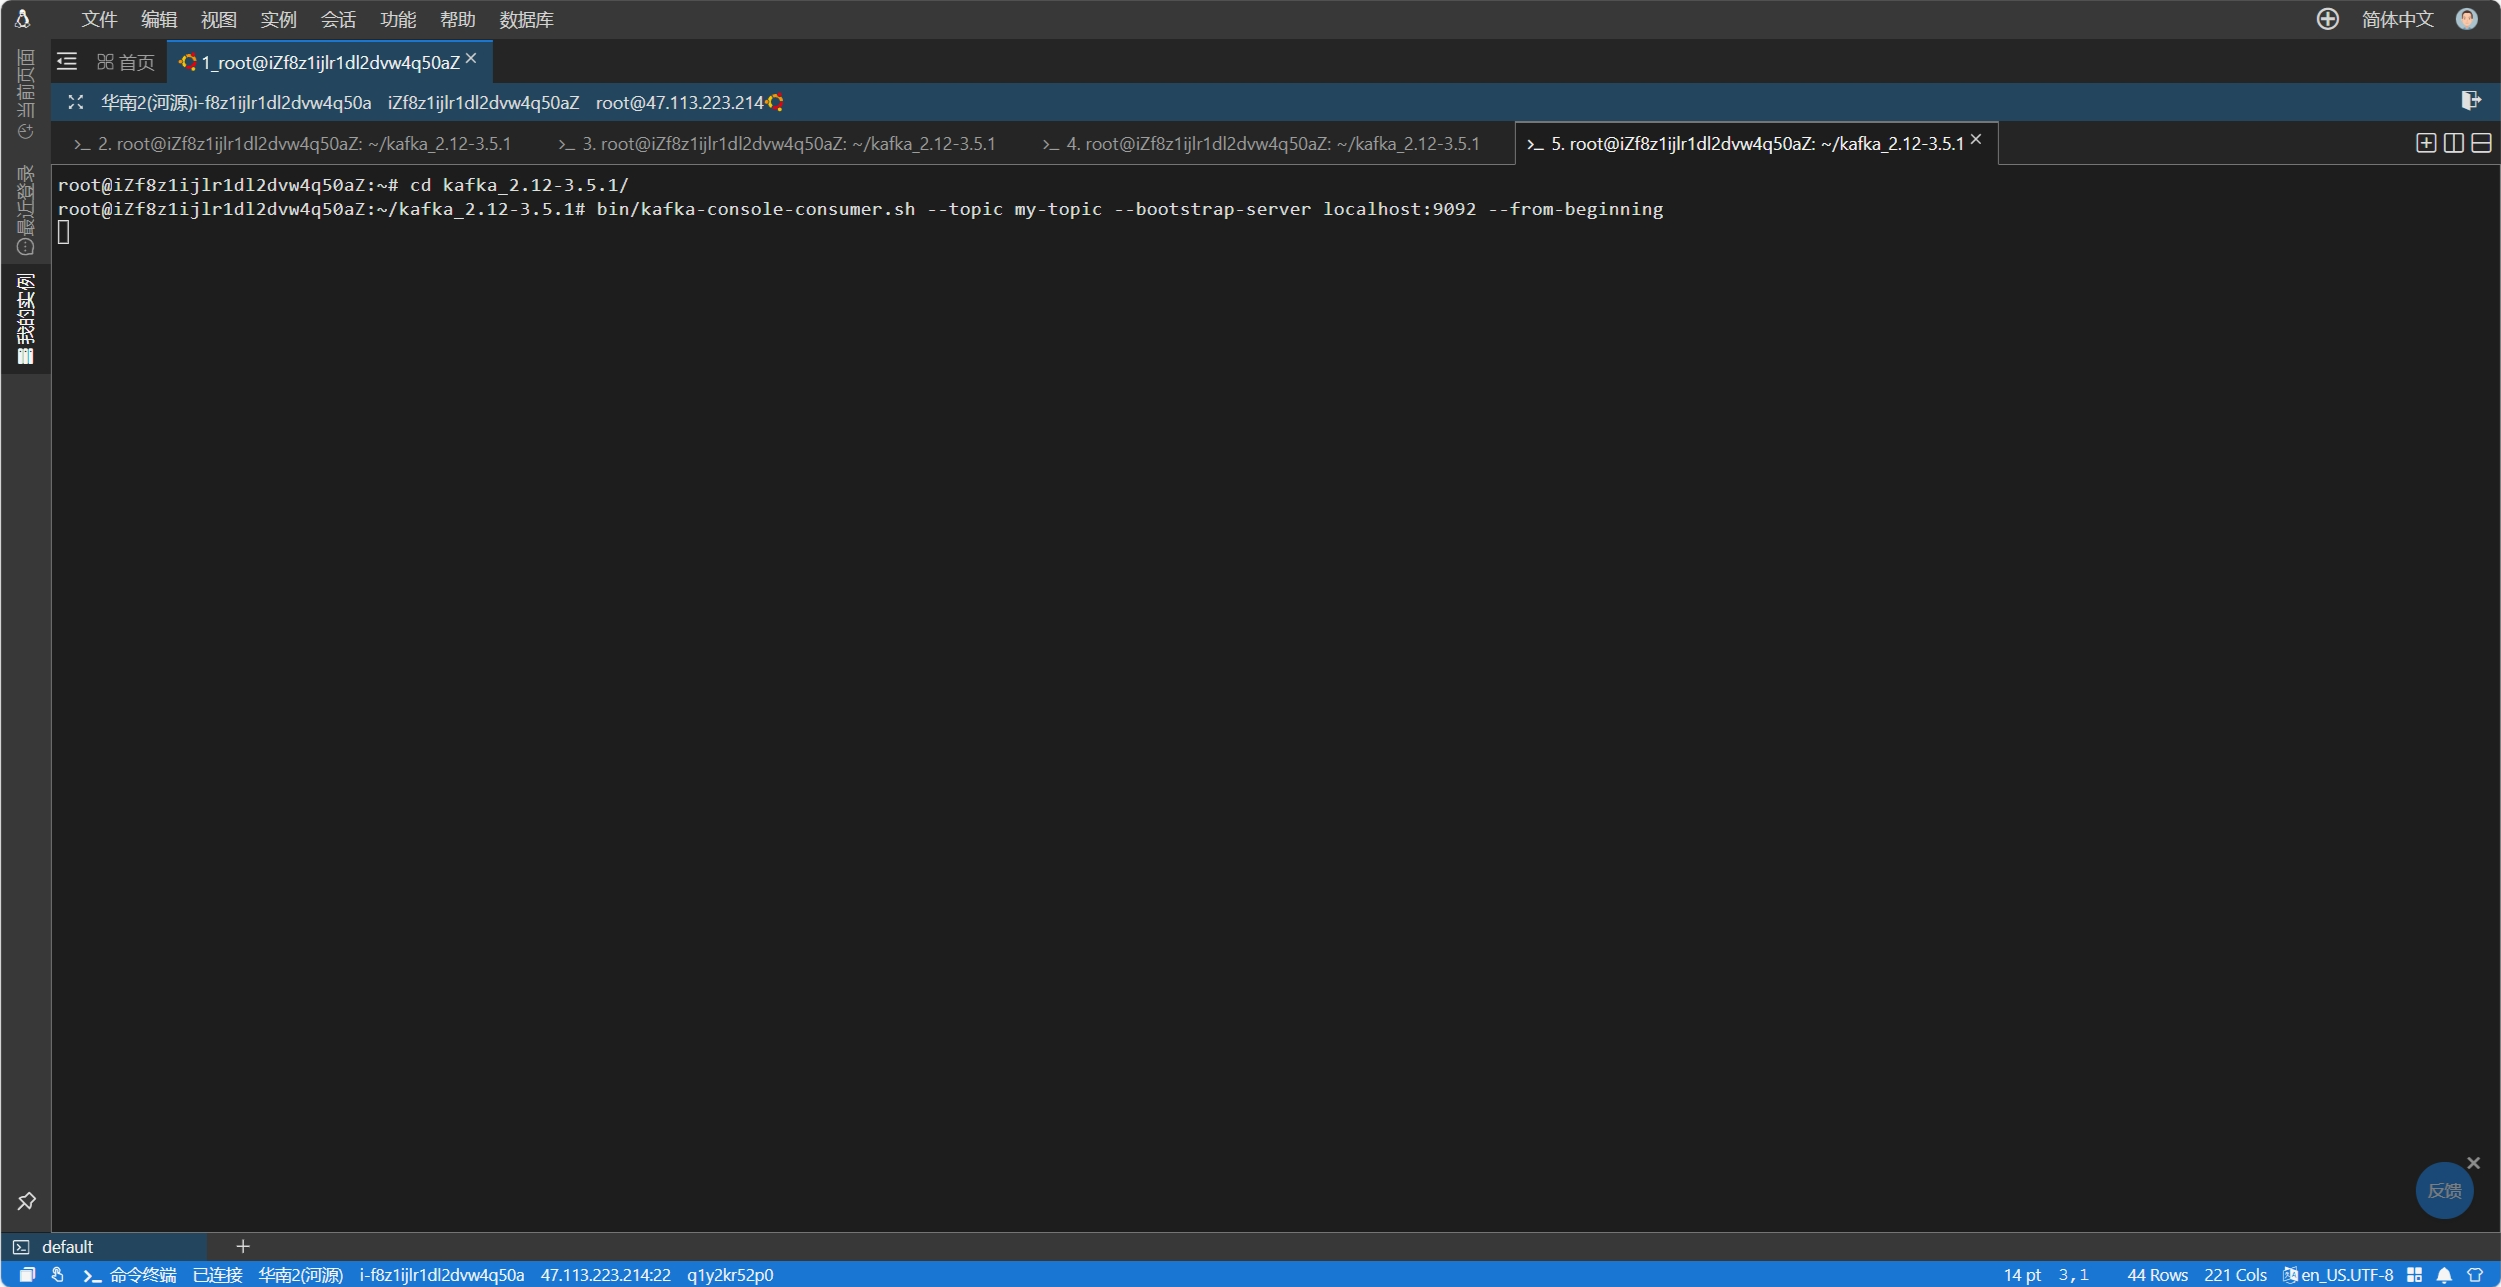
\includegraphics[width=0.7\textwidth]{./pic/7.png}
        \caption{创建消费者}
    \end{figure}
\end{itemize}
\subsection*{1.5 确认Kafka主题中的消息}
生产者生产消息,消费者消费消息
\begin{figure}[H]
    \centering
    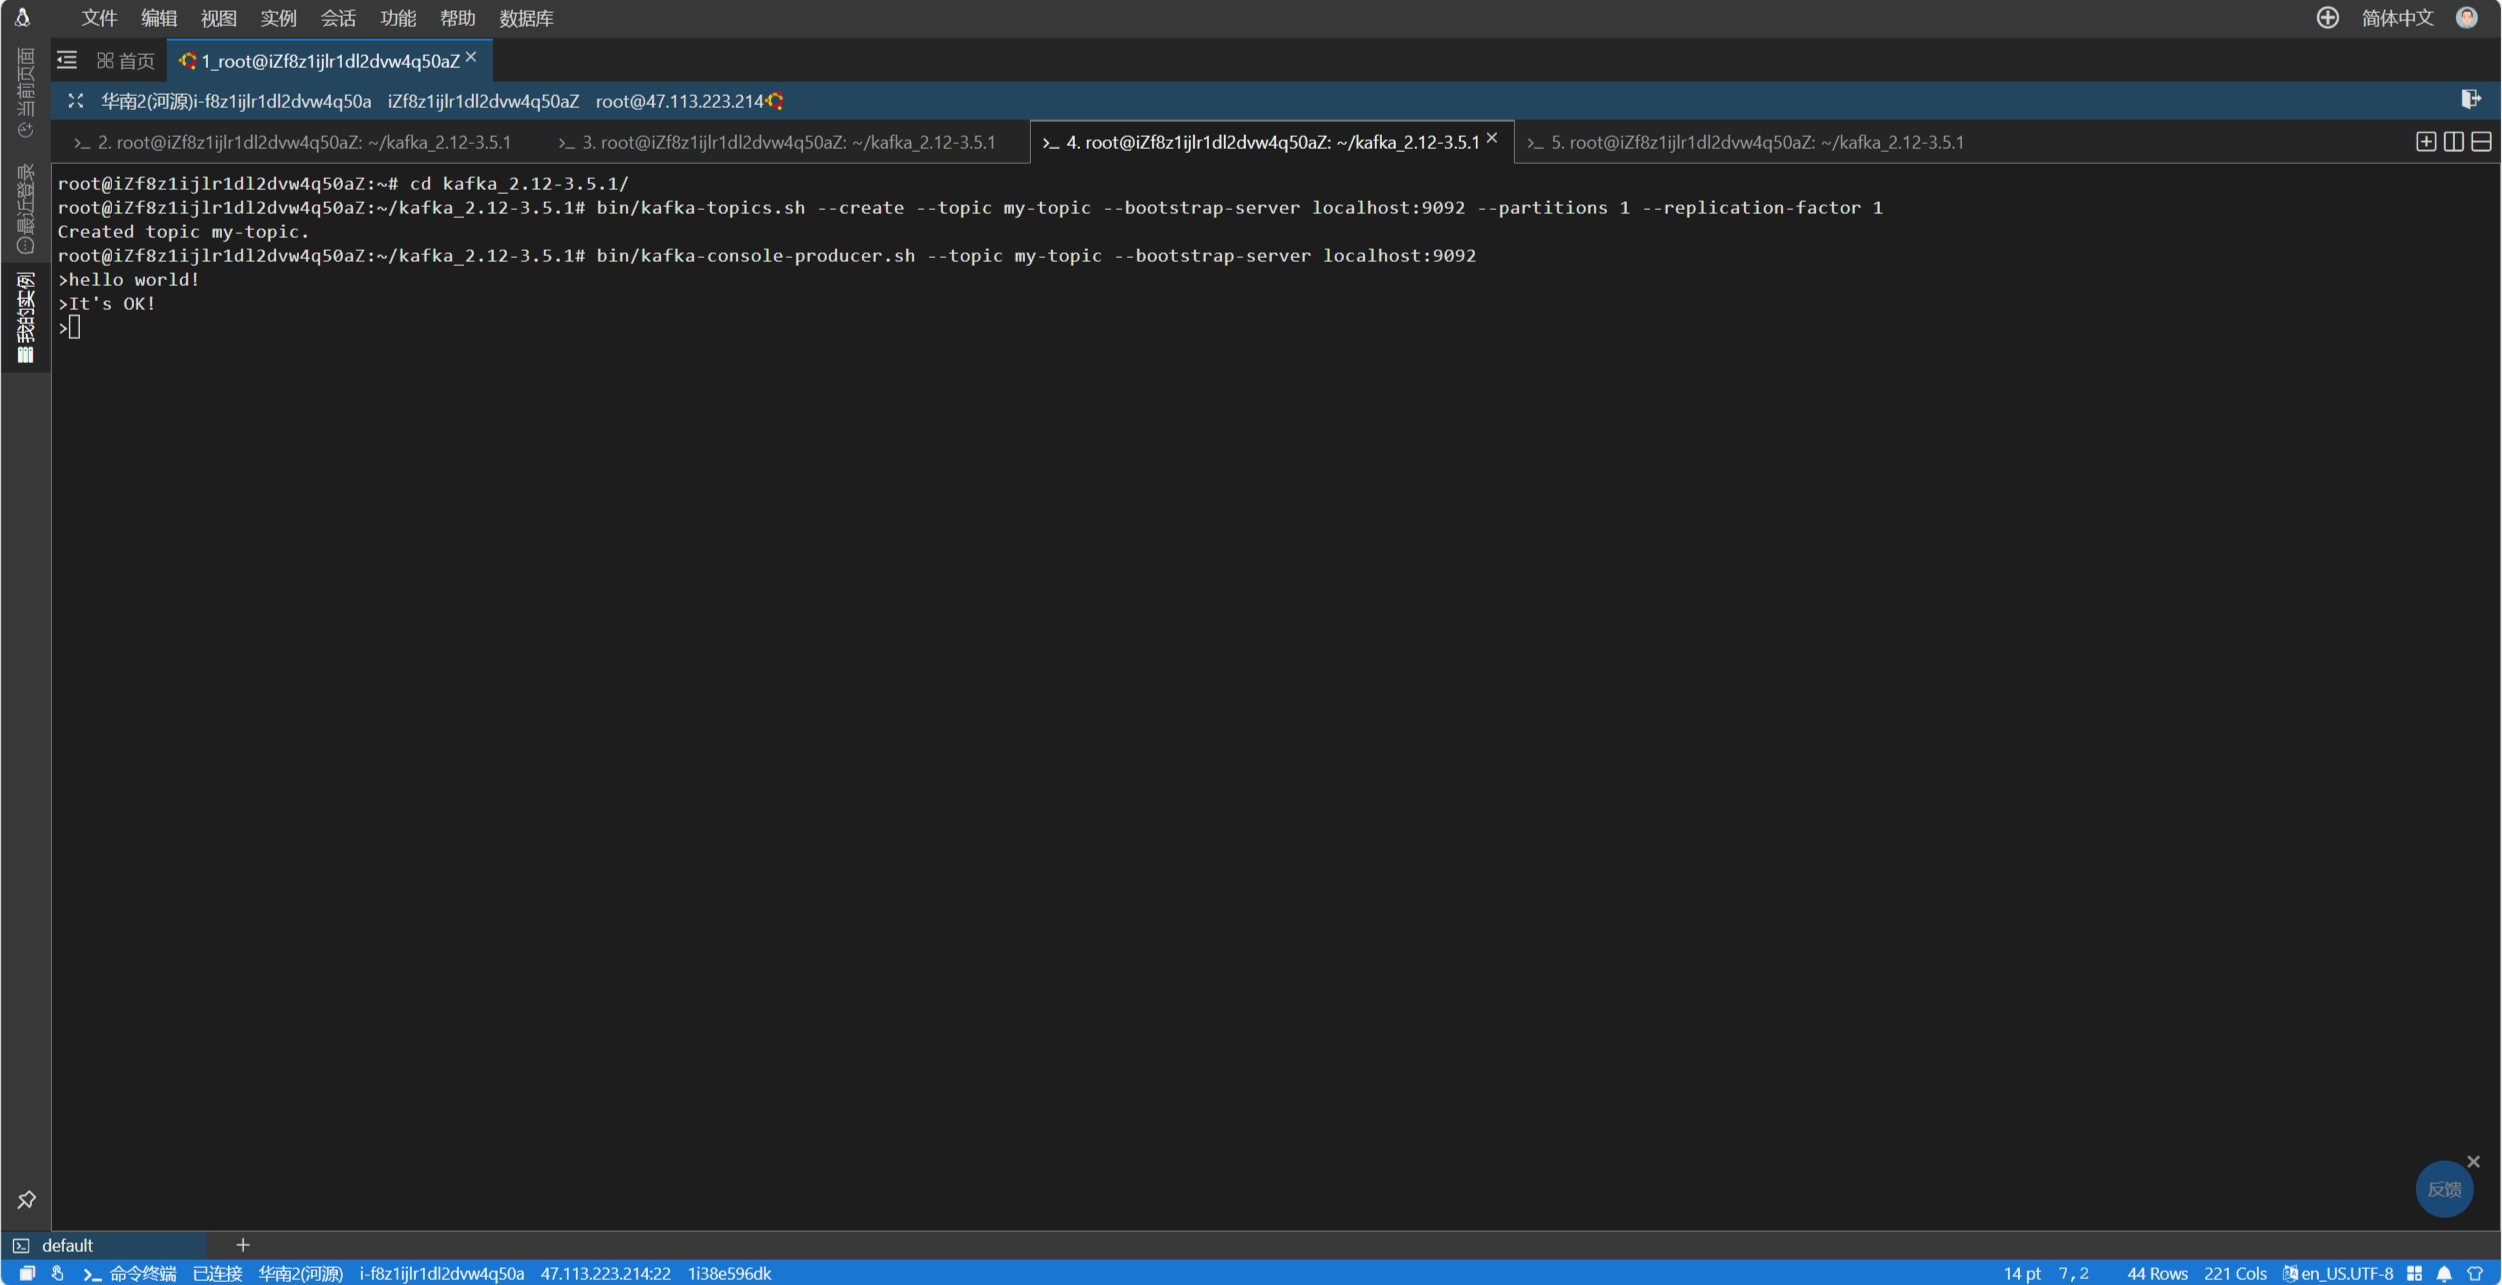
\includegraphics[width=0.7\textwidth]{./pic/8.png}
    \caption{生产消息}
\end{figure}
\begin{figure}[H]
    \centering
    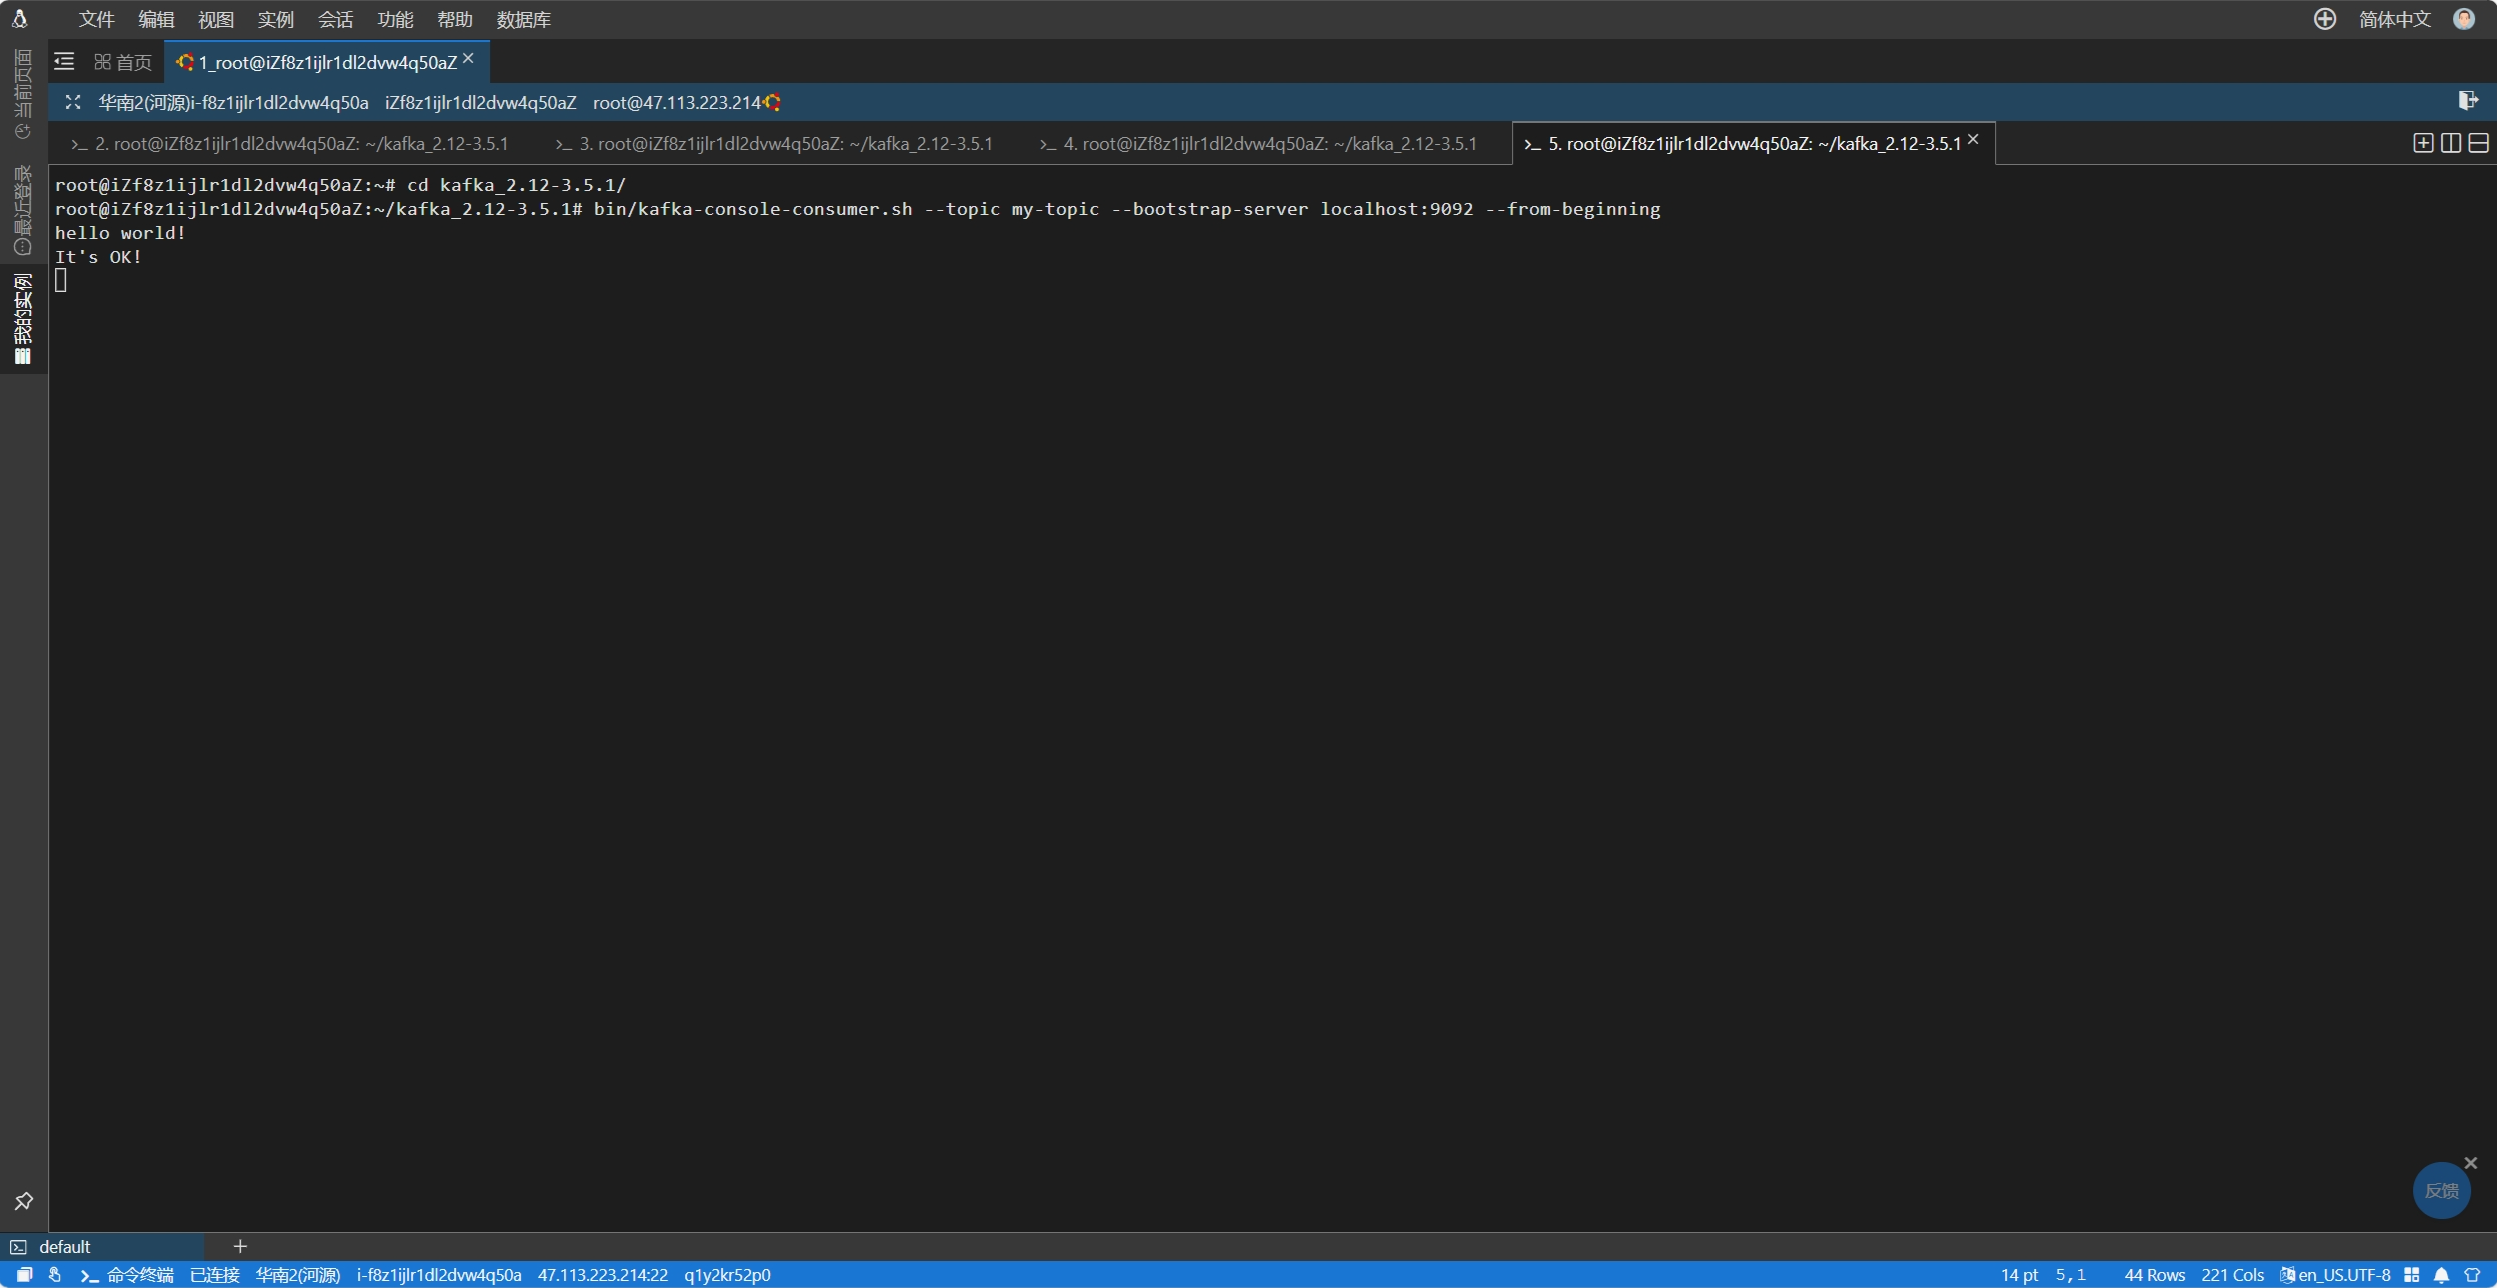
\includegraphics[width=0.7\textwidth]{./pic/9.png}
    \caption{消费消息}
\end{figure}

\section{任务4:使用Flume收集日志}
\subsection*{1.1 安装Flume}
通过\lstinline[style=Style]|wget https://mirrors.aliyun.com/apache/flume/1.11.0/apache-flume-1.11.0-bin.tar.gz|获取Flume并解压至flume-1.11.0.
\begin{figure}[H]
    \centering
    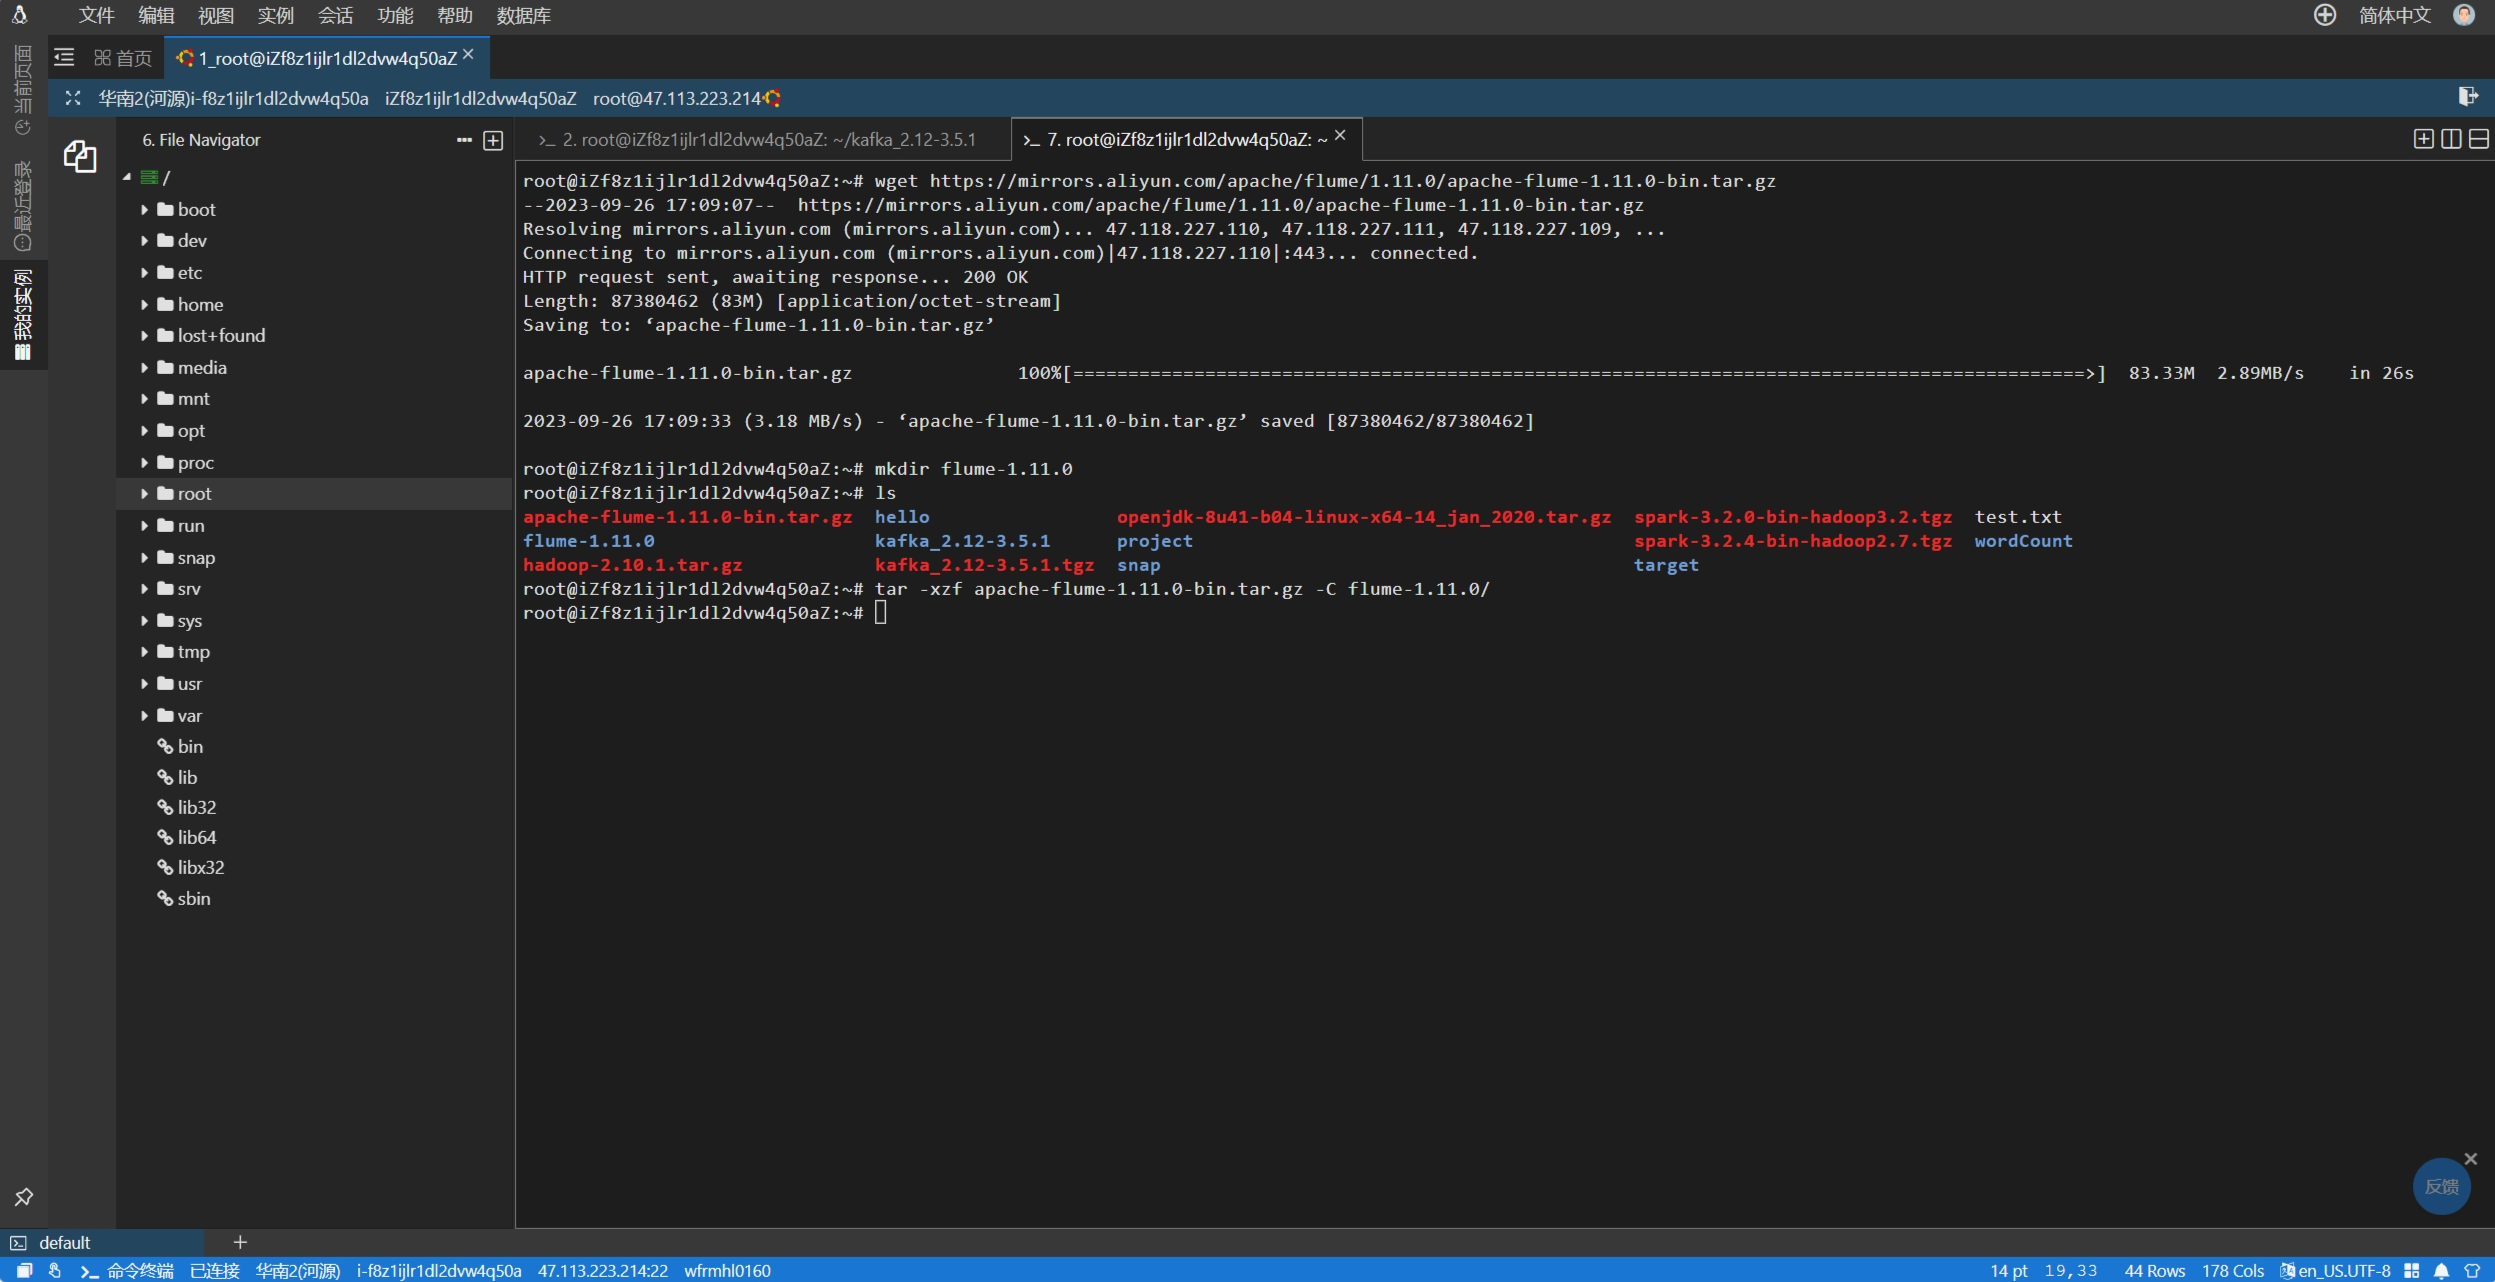
\includegraphics[width=0.7\textwidth]{./pic/12.png}
    \caption{安装Flume}
\end{figure}
通过\lstinline[style=Style]|bin/flume-ng version|查看是否安装成功。
\begin{figure}[H]
    \centering
    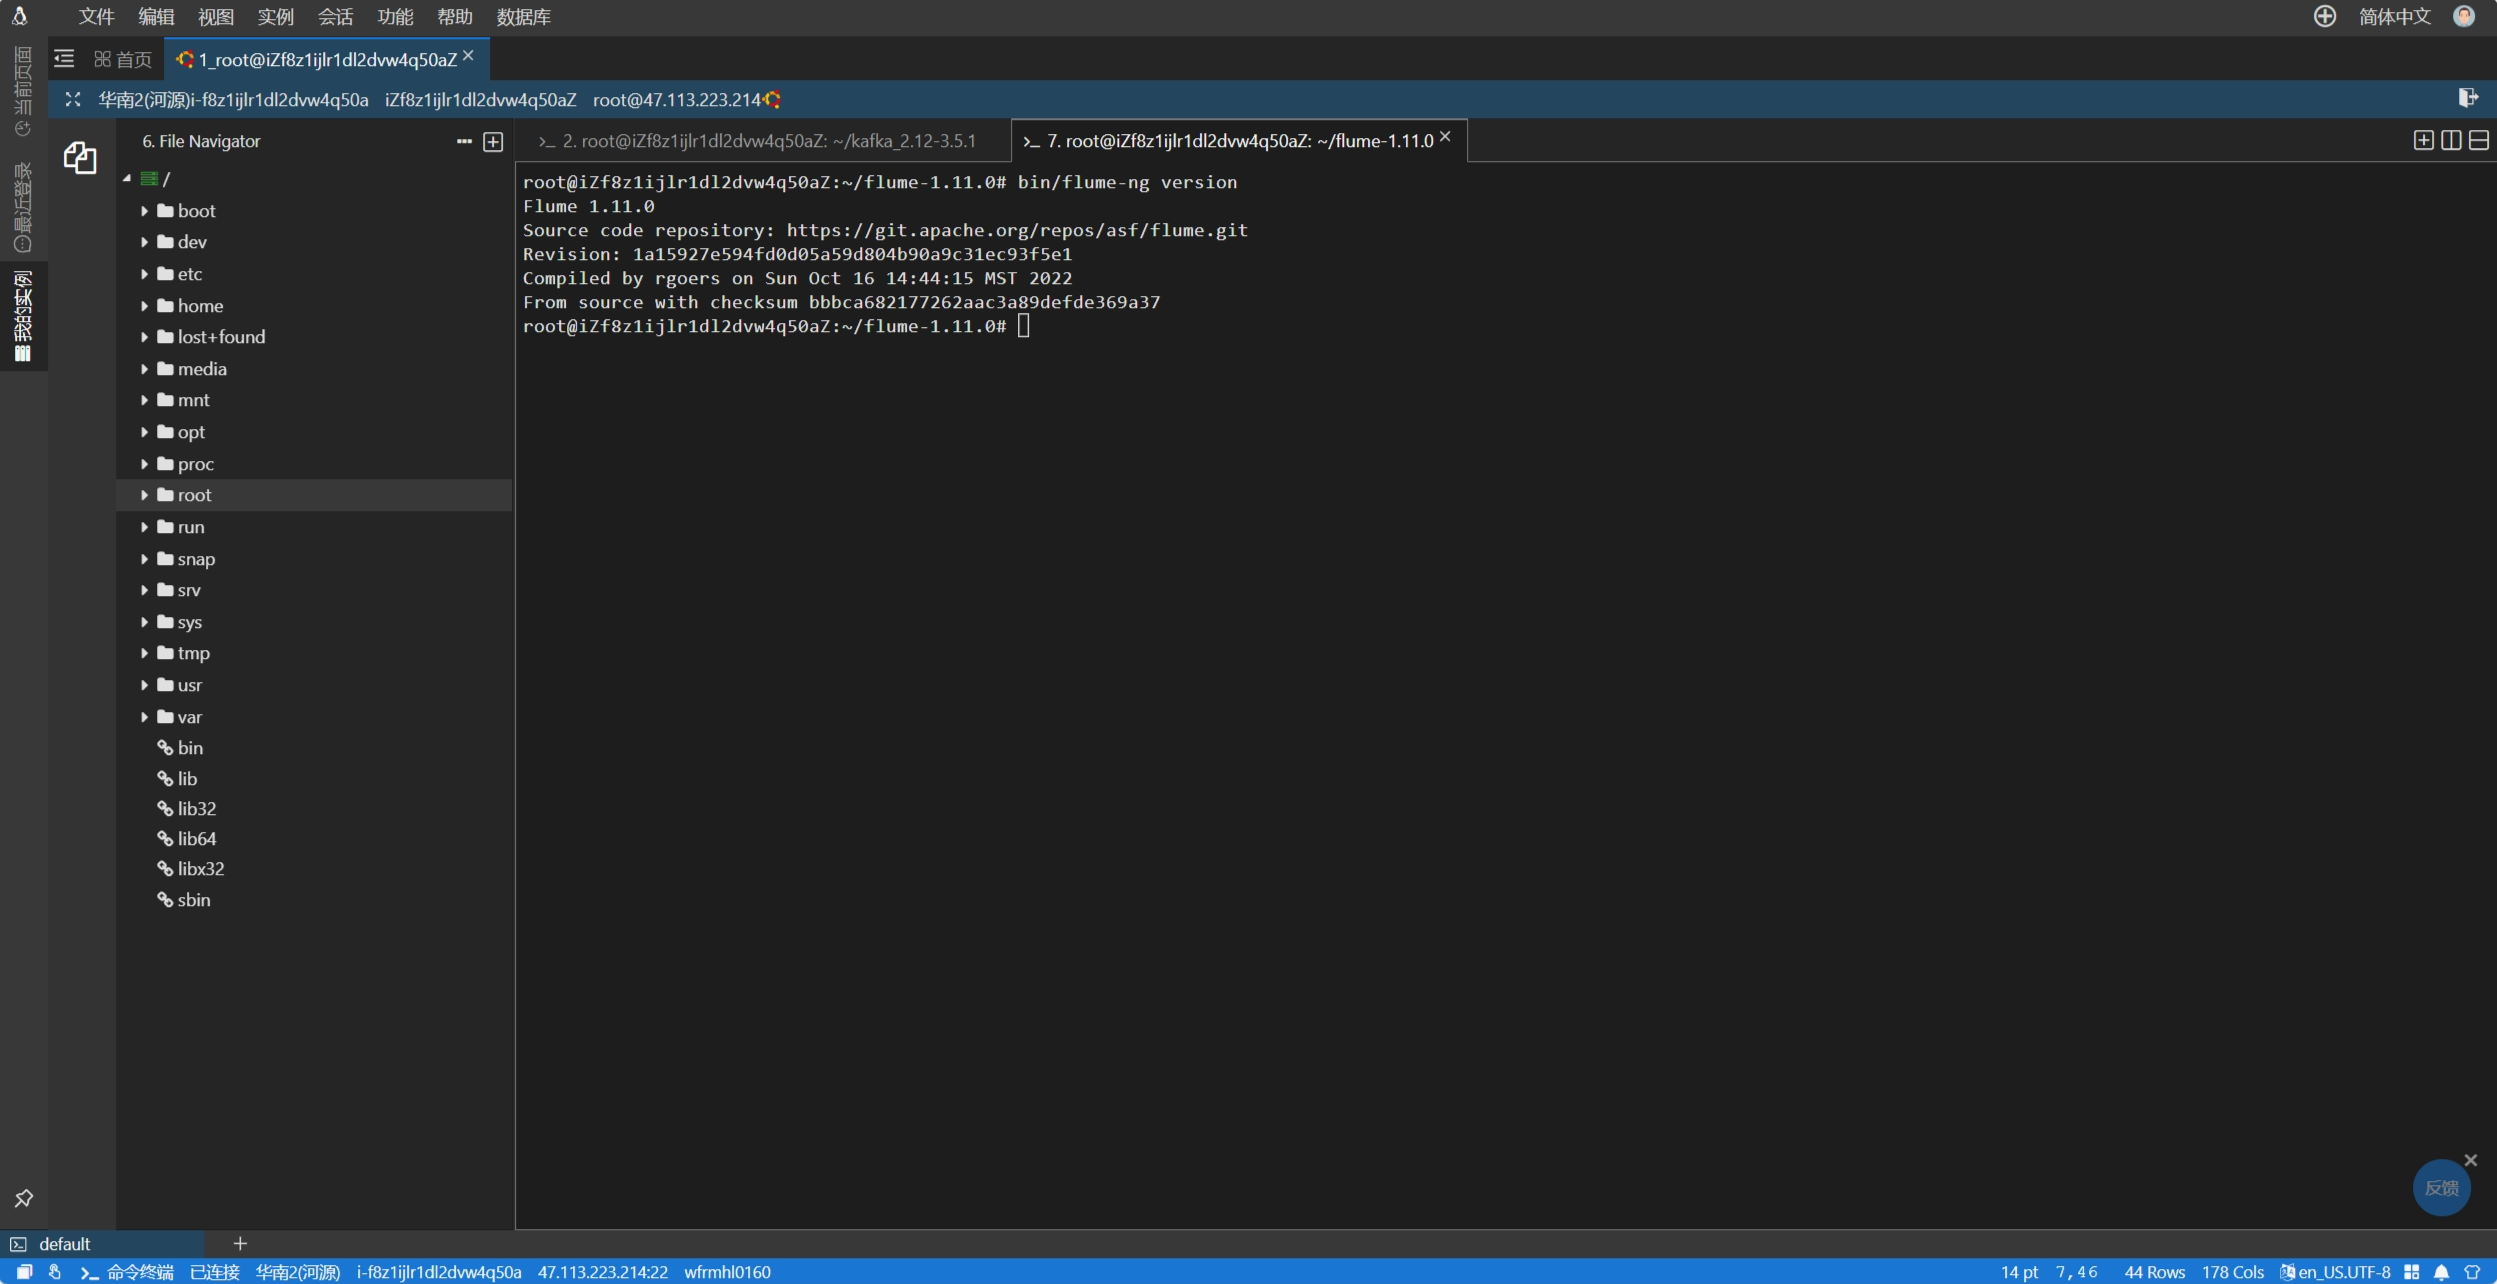
\includegraphics[width=0.7\textwidth]{./pic/13.png}
    \caption{查看Flume版本}
\end{figure}
\subsection*{1.2 启动Hadoop}
Hadoop环境已经在实验2中配置完成。
\begin{figure}[H]
    \centering
    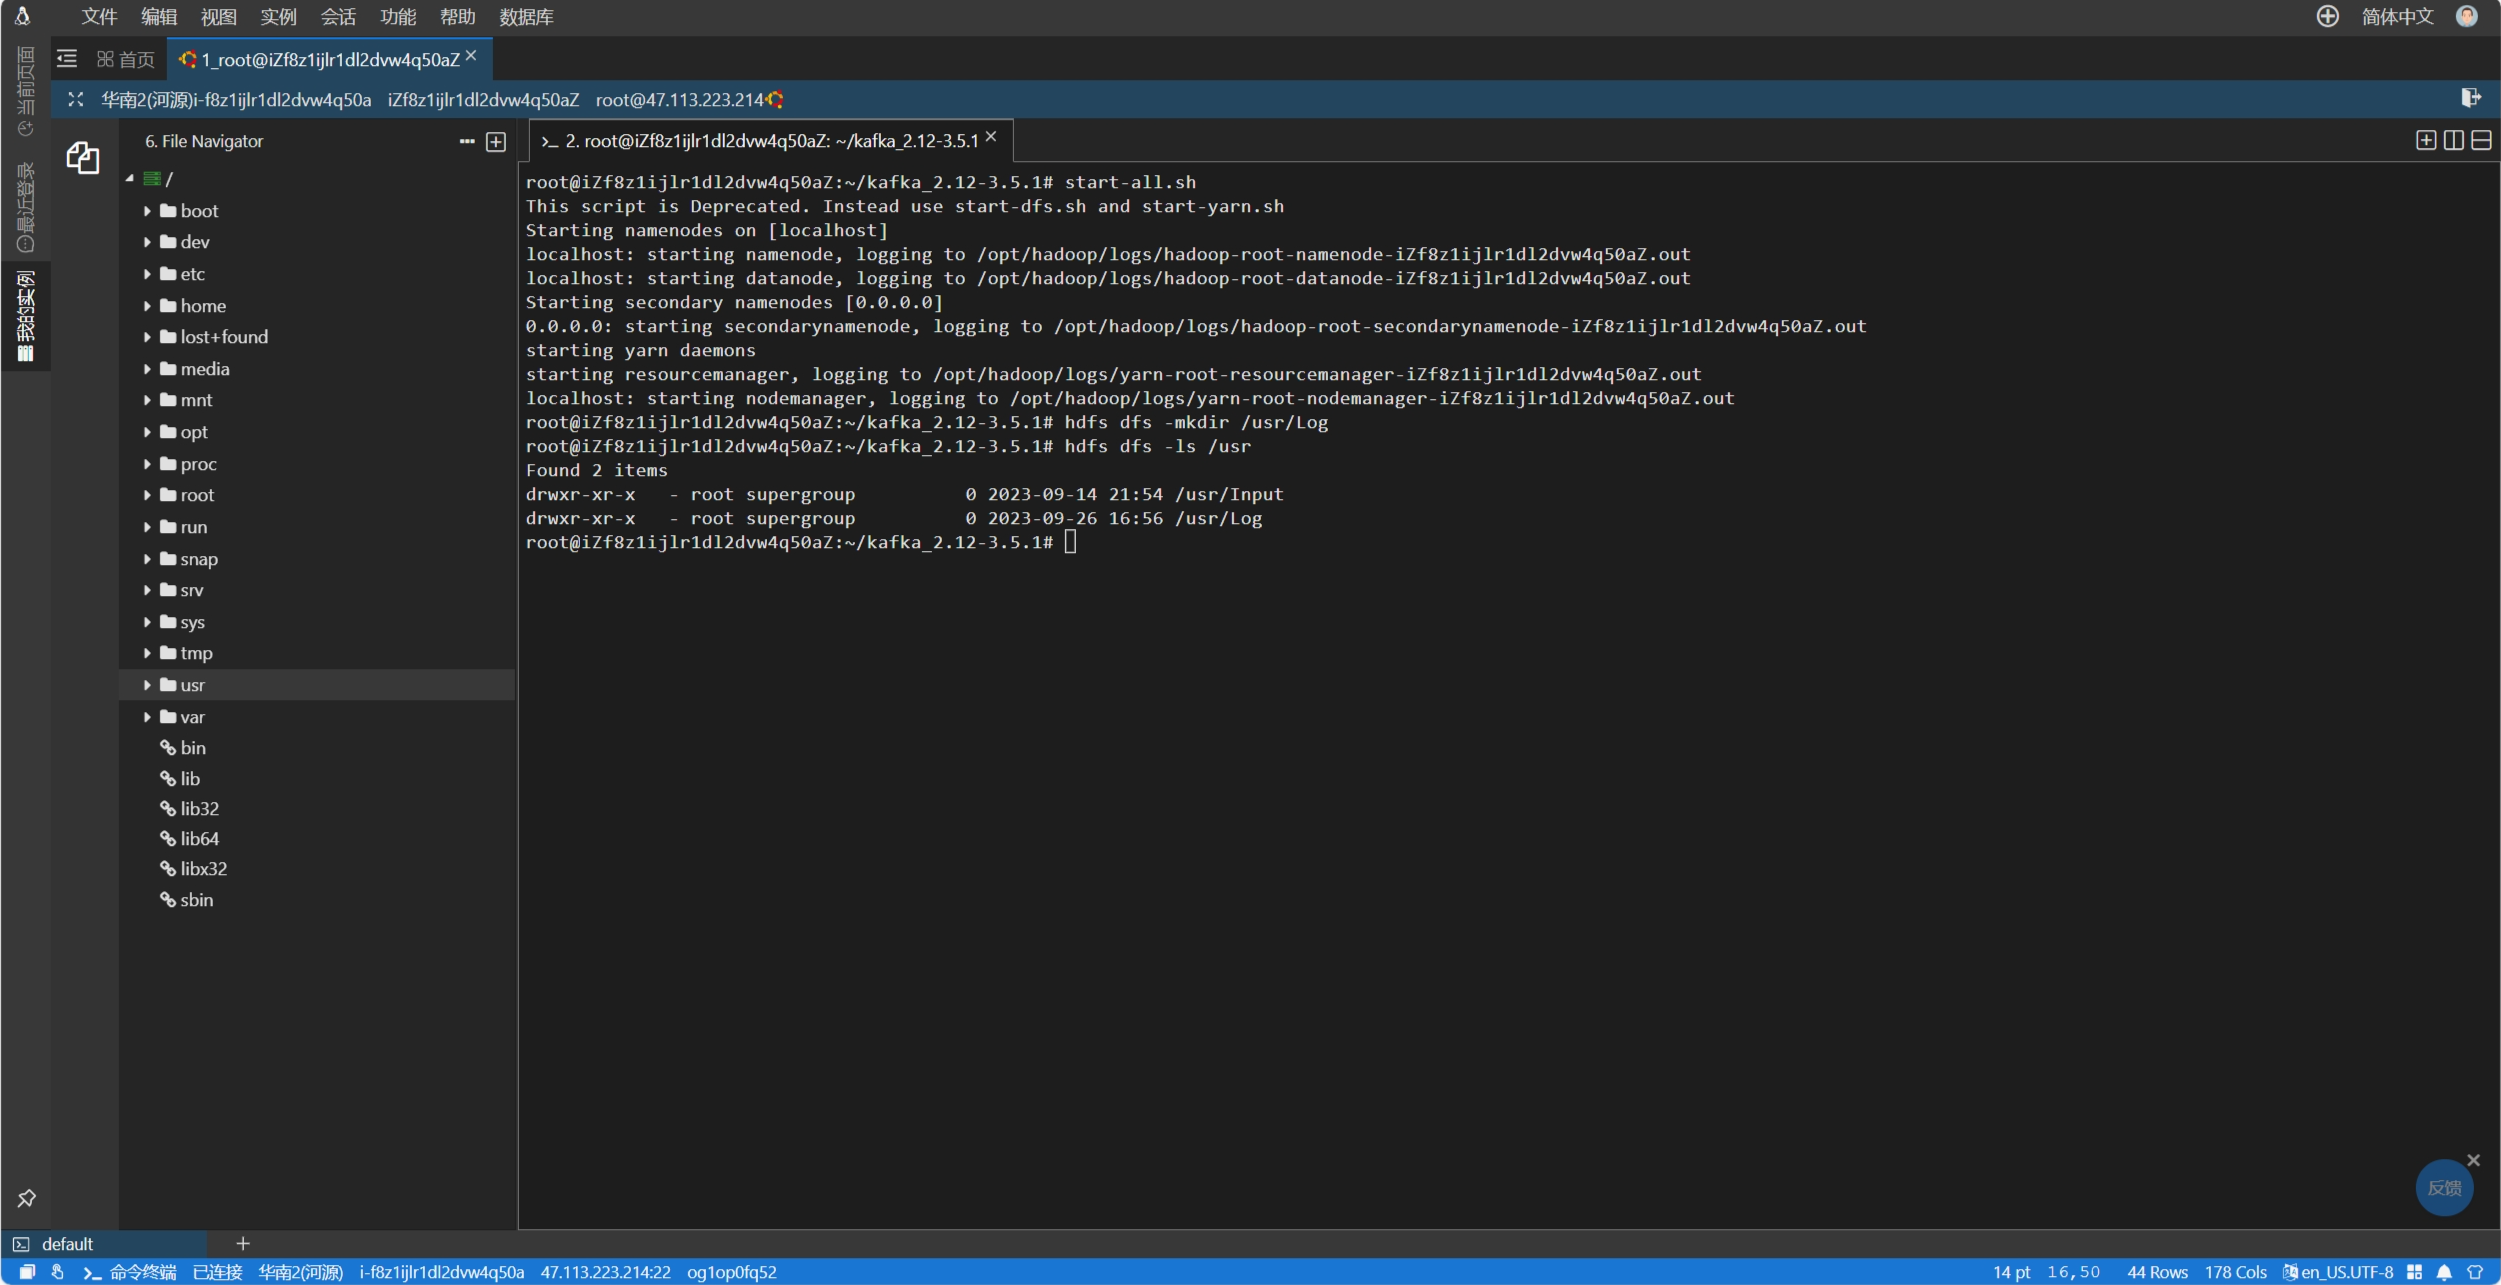
\includegraphics[width=0.35\textwidth]{./pic/10.png}
    \caption{启动Hadoop}
\end{figure}
\subsection*{1.3 配置Flume}
配置文件的内容如下:
\begin{figure}[H]
    \centering
    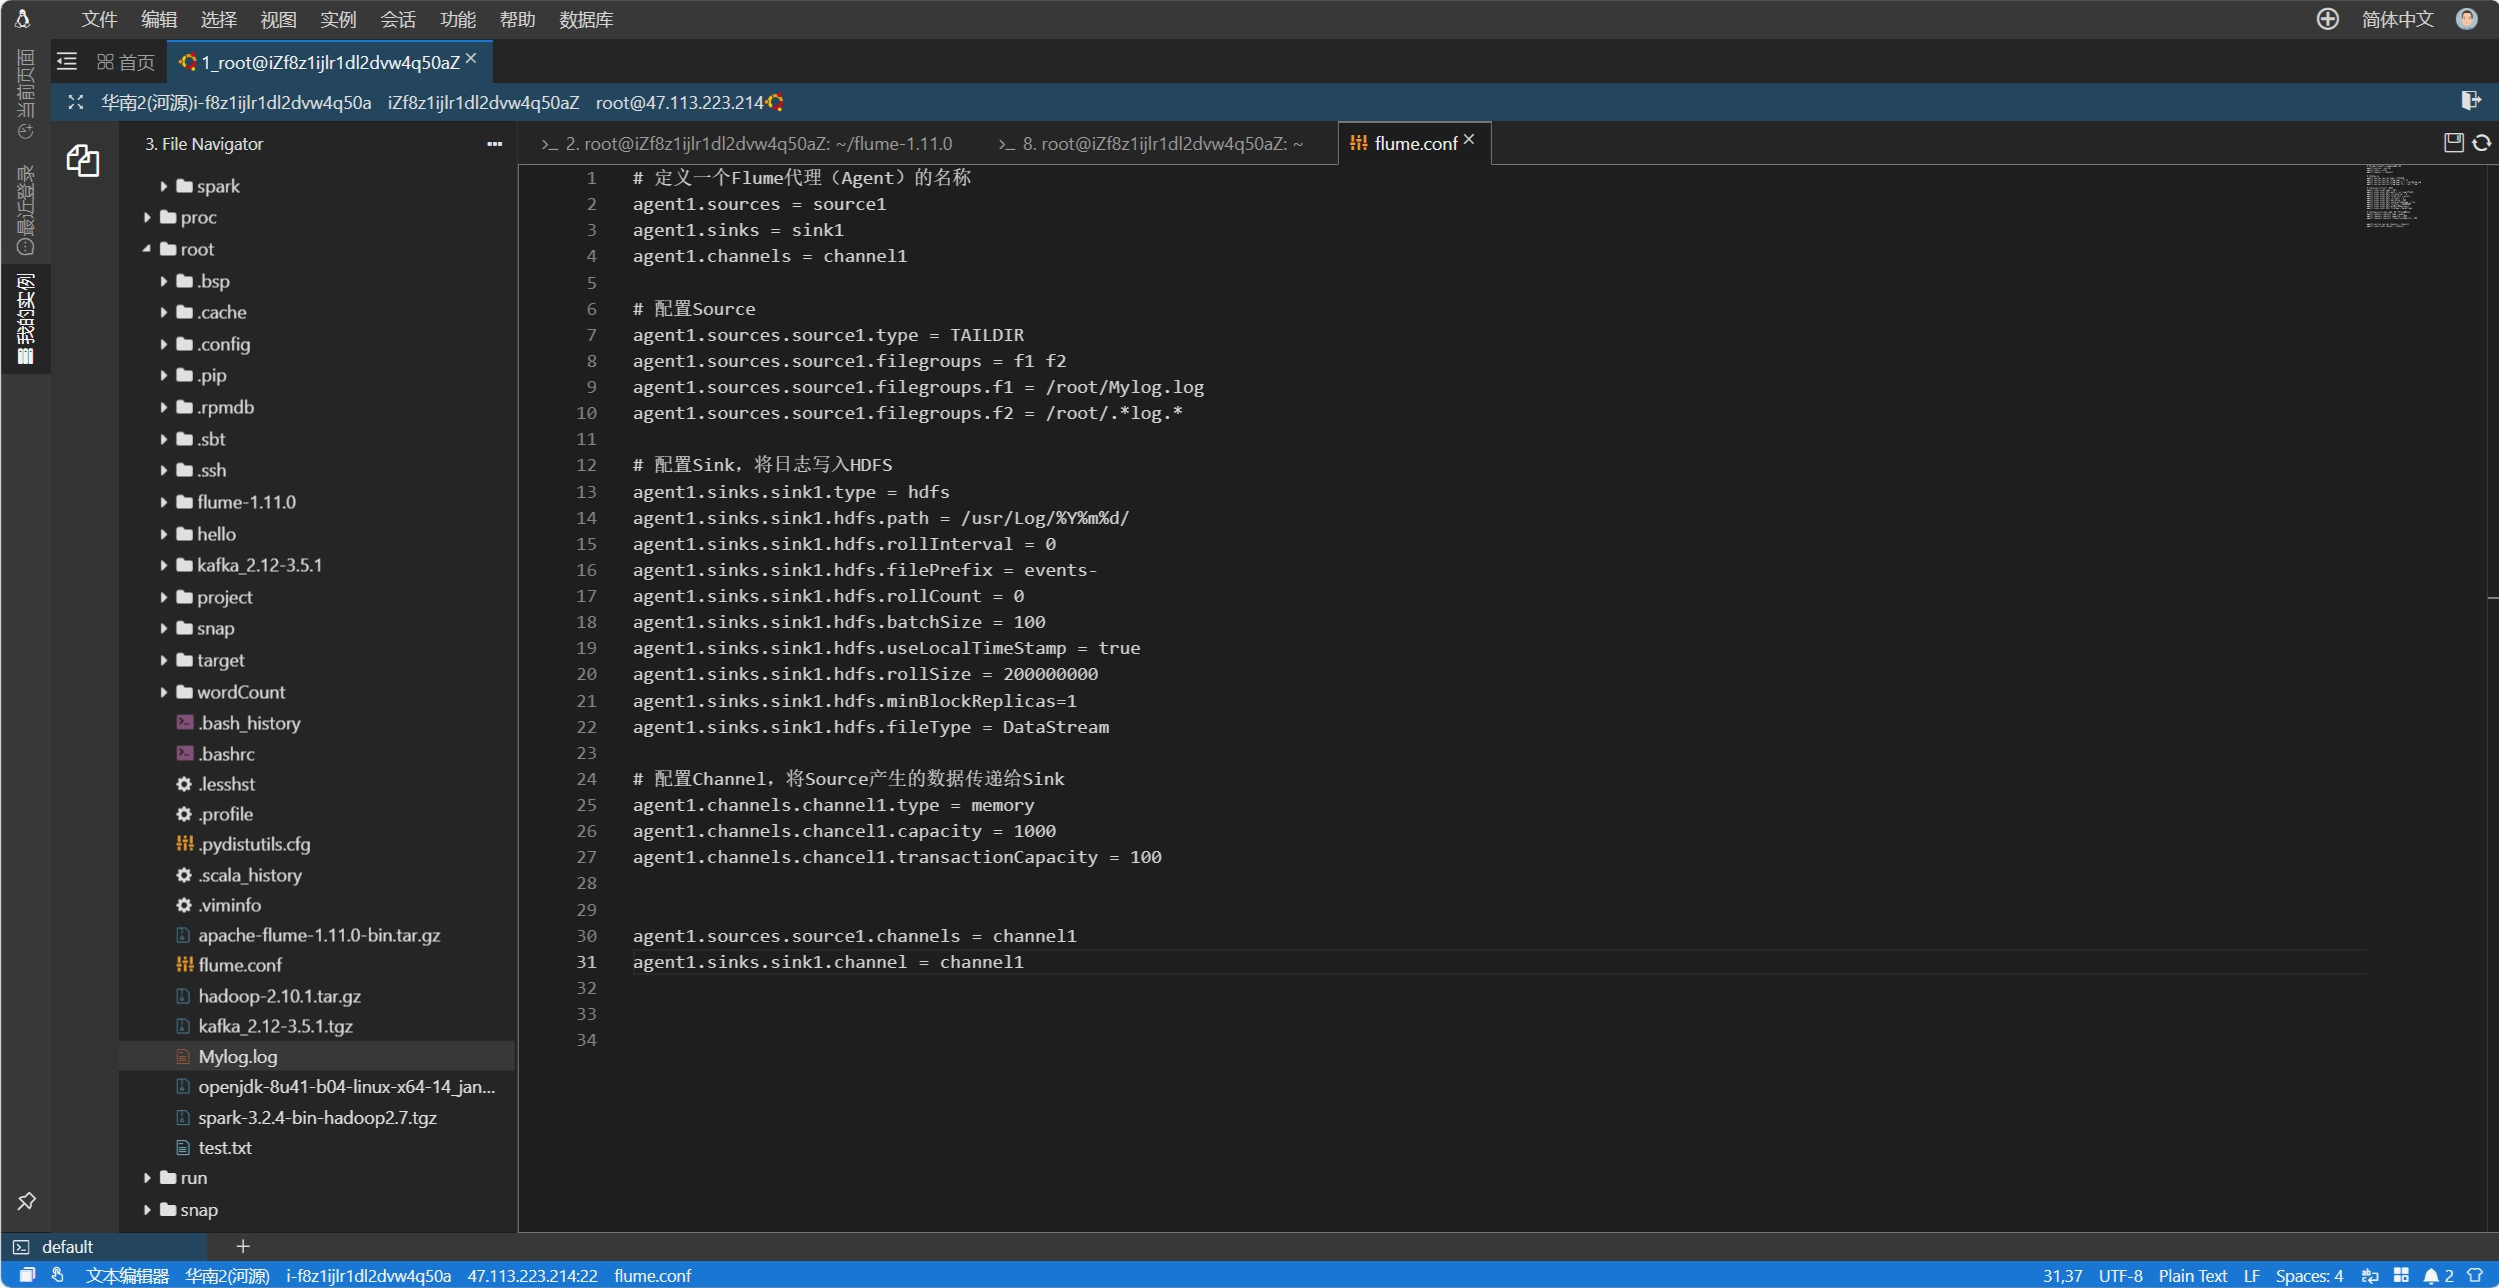
\includegraphics[width=0.7\textwidth]{./pic/14.png}
    \caption{flume.conf}
\end{figure}
\subsection*{1.4 启动Flume}
完成配置后,可以启动Flume代理来开始日志收集和传输。使用以下命令启动Flume:\par
\lstinline[style=Style]|bin/flume-ng agent --conf conf --conf-file /root/flume.conf -name agent1 -Dflume.root.logger=INFO,console|
\begin{figure}[H]
    \centering
    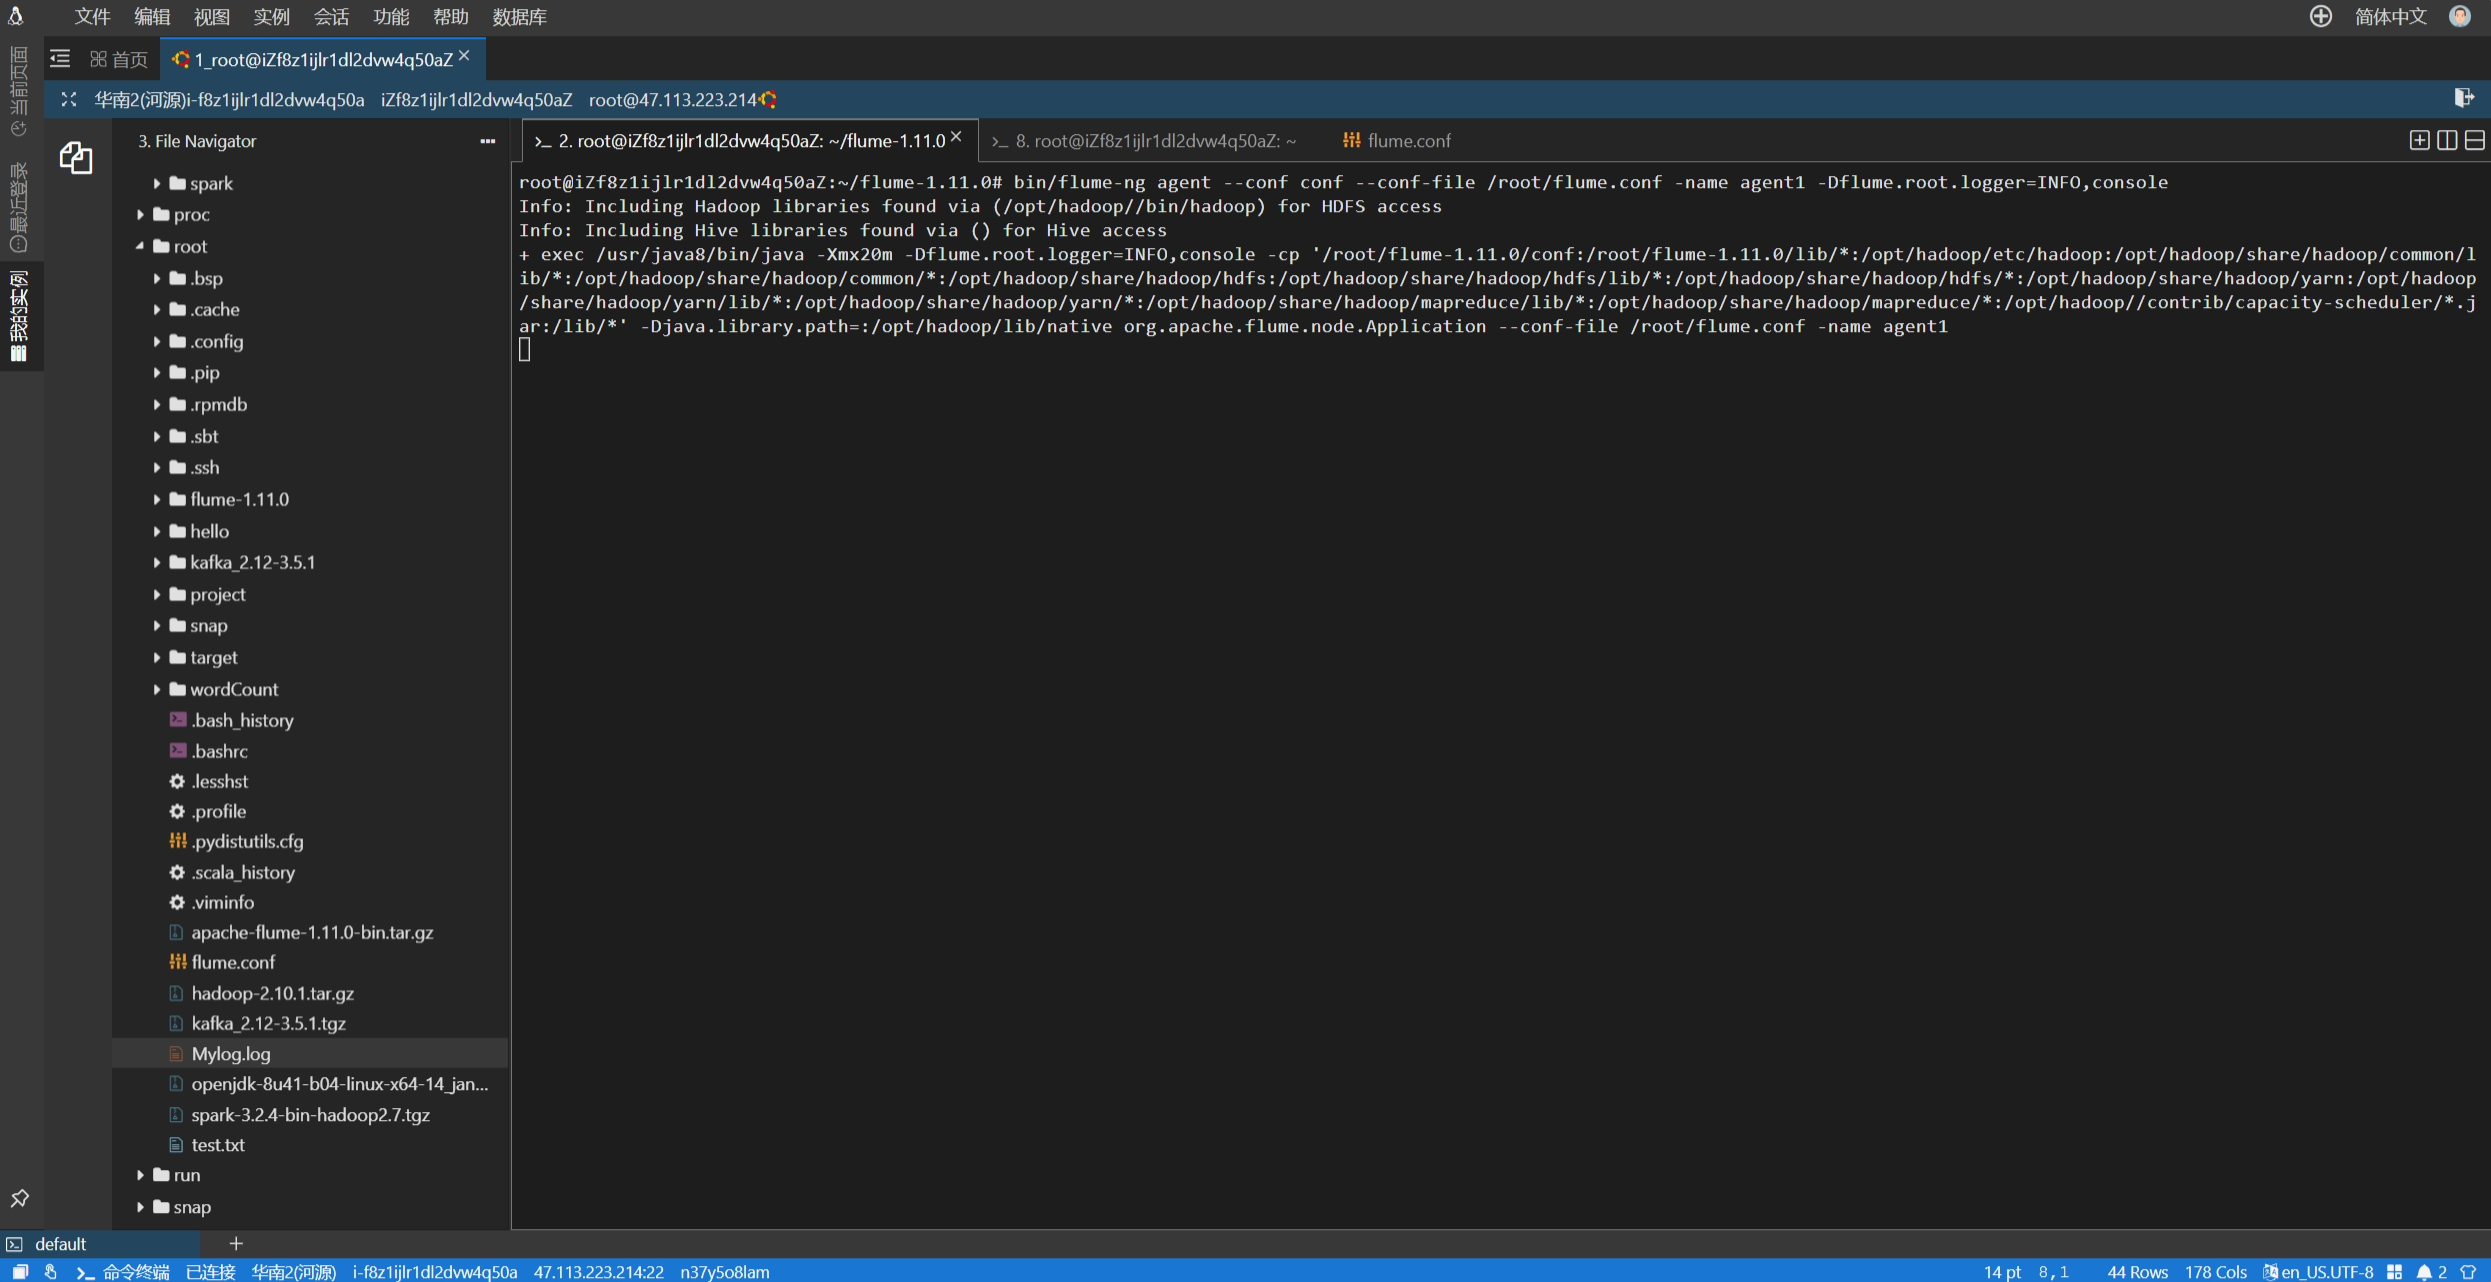
\includegraphics[width=0.7\textwidth]{./pic/16.png}
    \caption{启动Flume}
\end{figure}
\subsection*{1.5 验证日志存储在HDFS中}
\begin{itemize}
    \item 在root目录下新建Mylog.log文件。
    \begin{figure}[H]
        \centering
        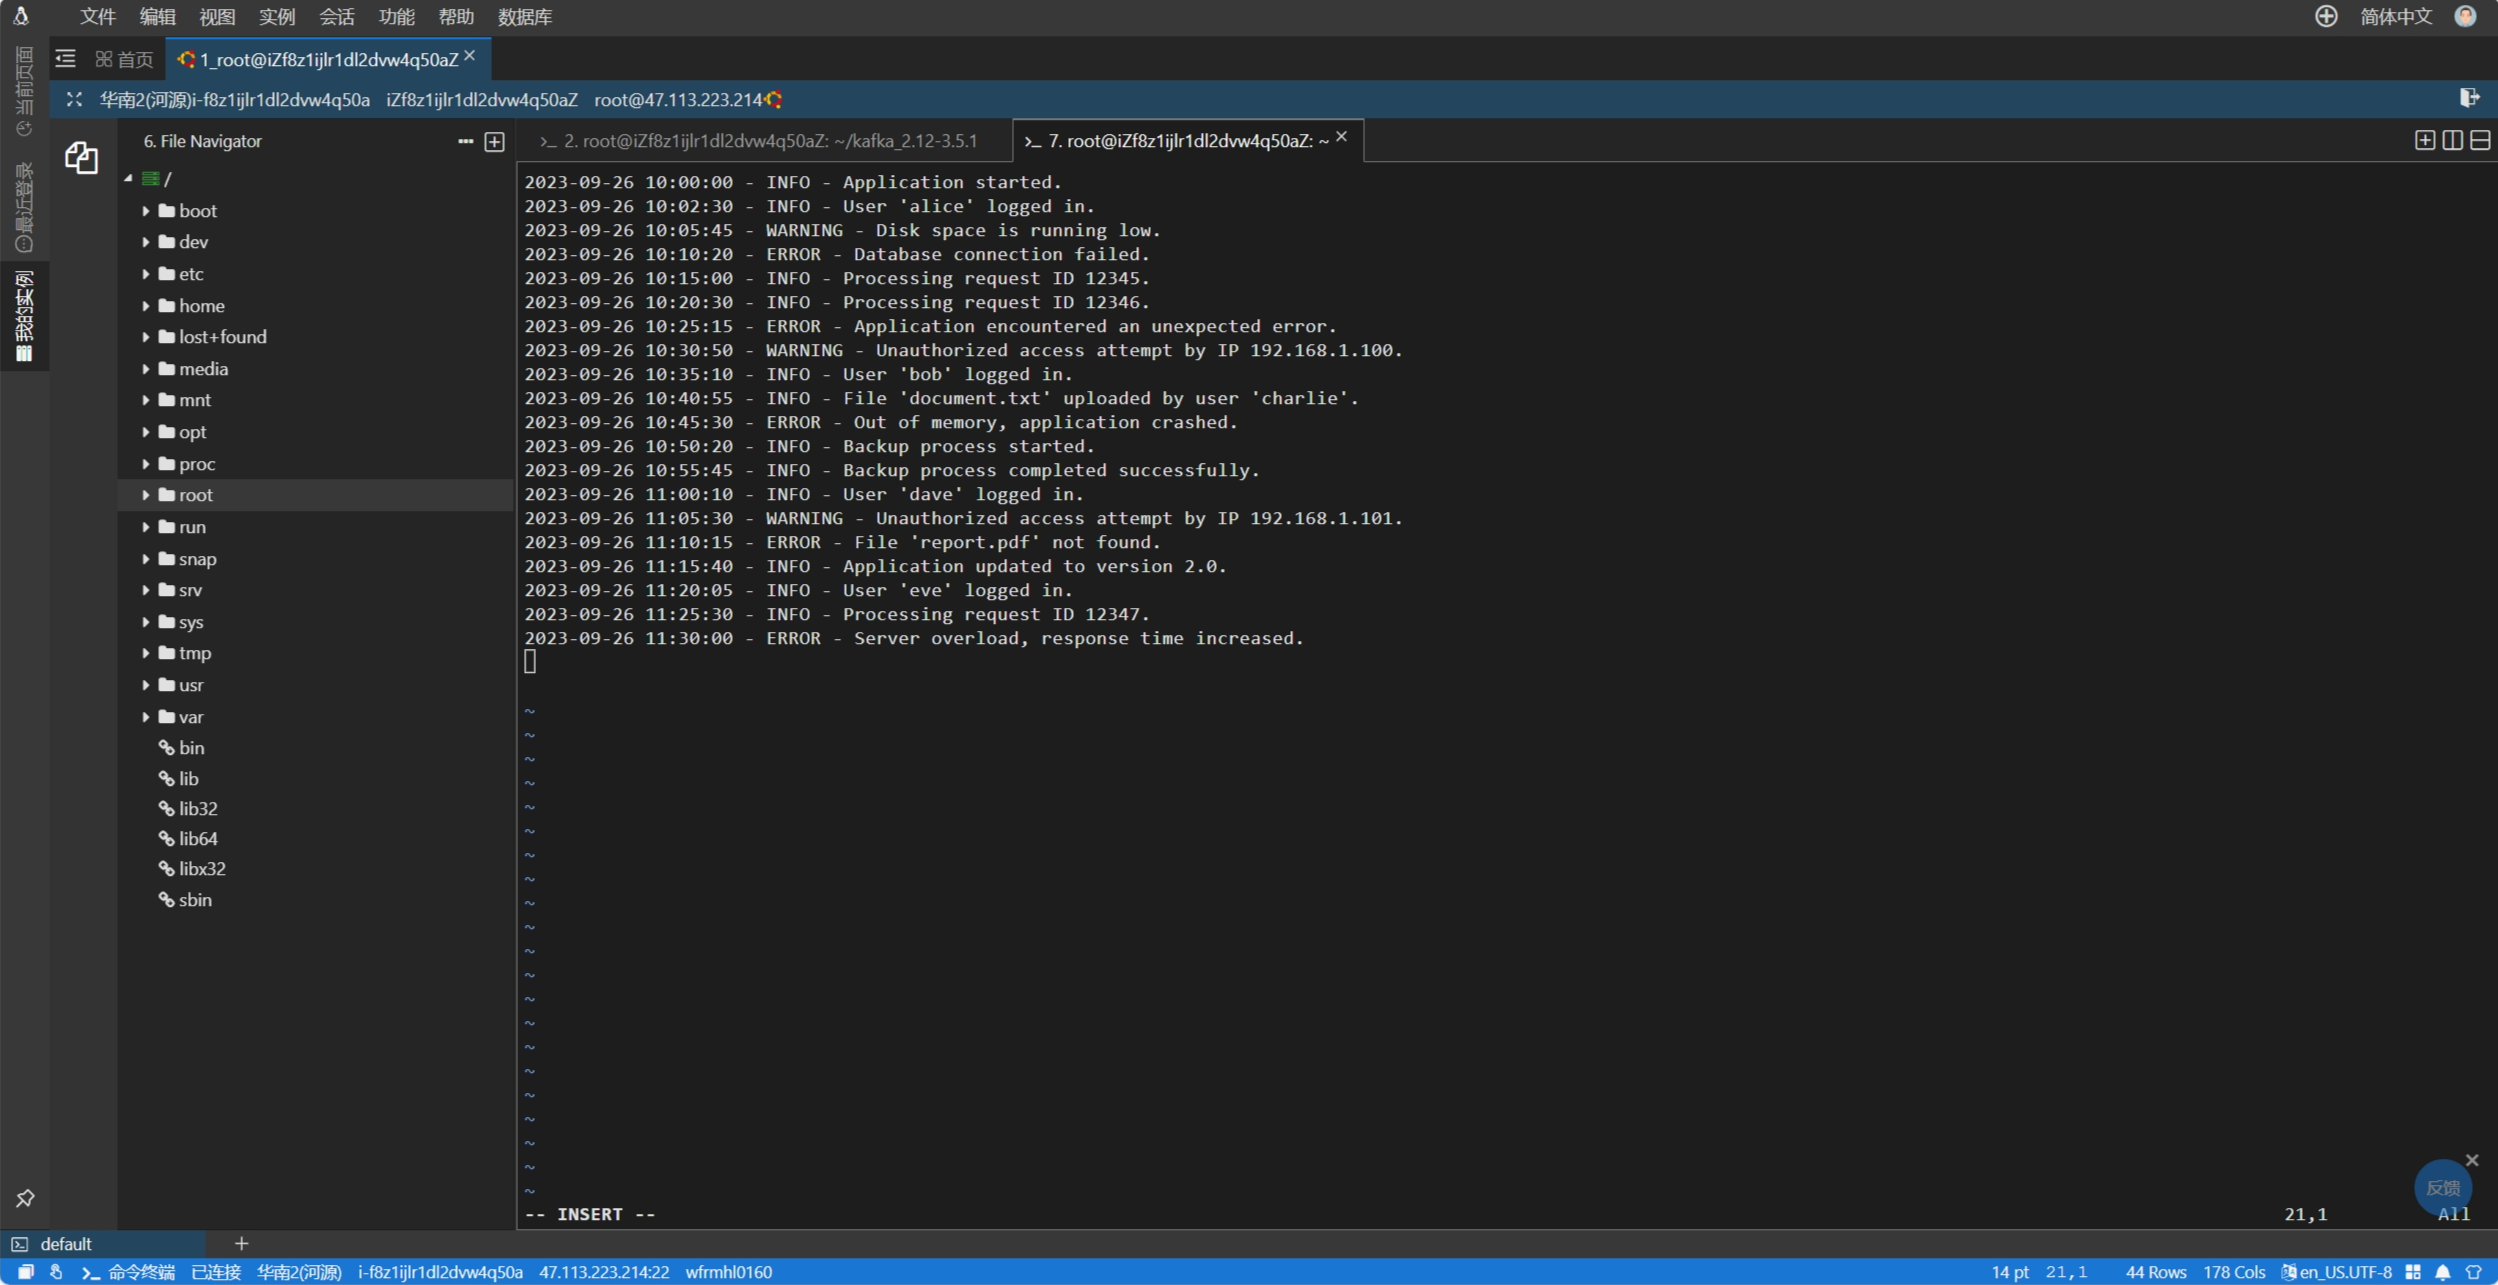
\includegraphics[width=0.7\textwidth]{./pic/15.png}
        \caption{Mylog.log}
    \end{figure}
    \item 在Hadoop的web界面查看,可以看到存储的日志。
    \begin{figure}[H]
        \centering
        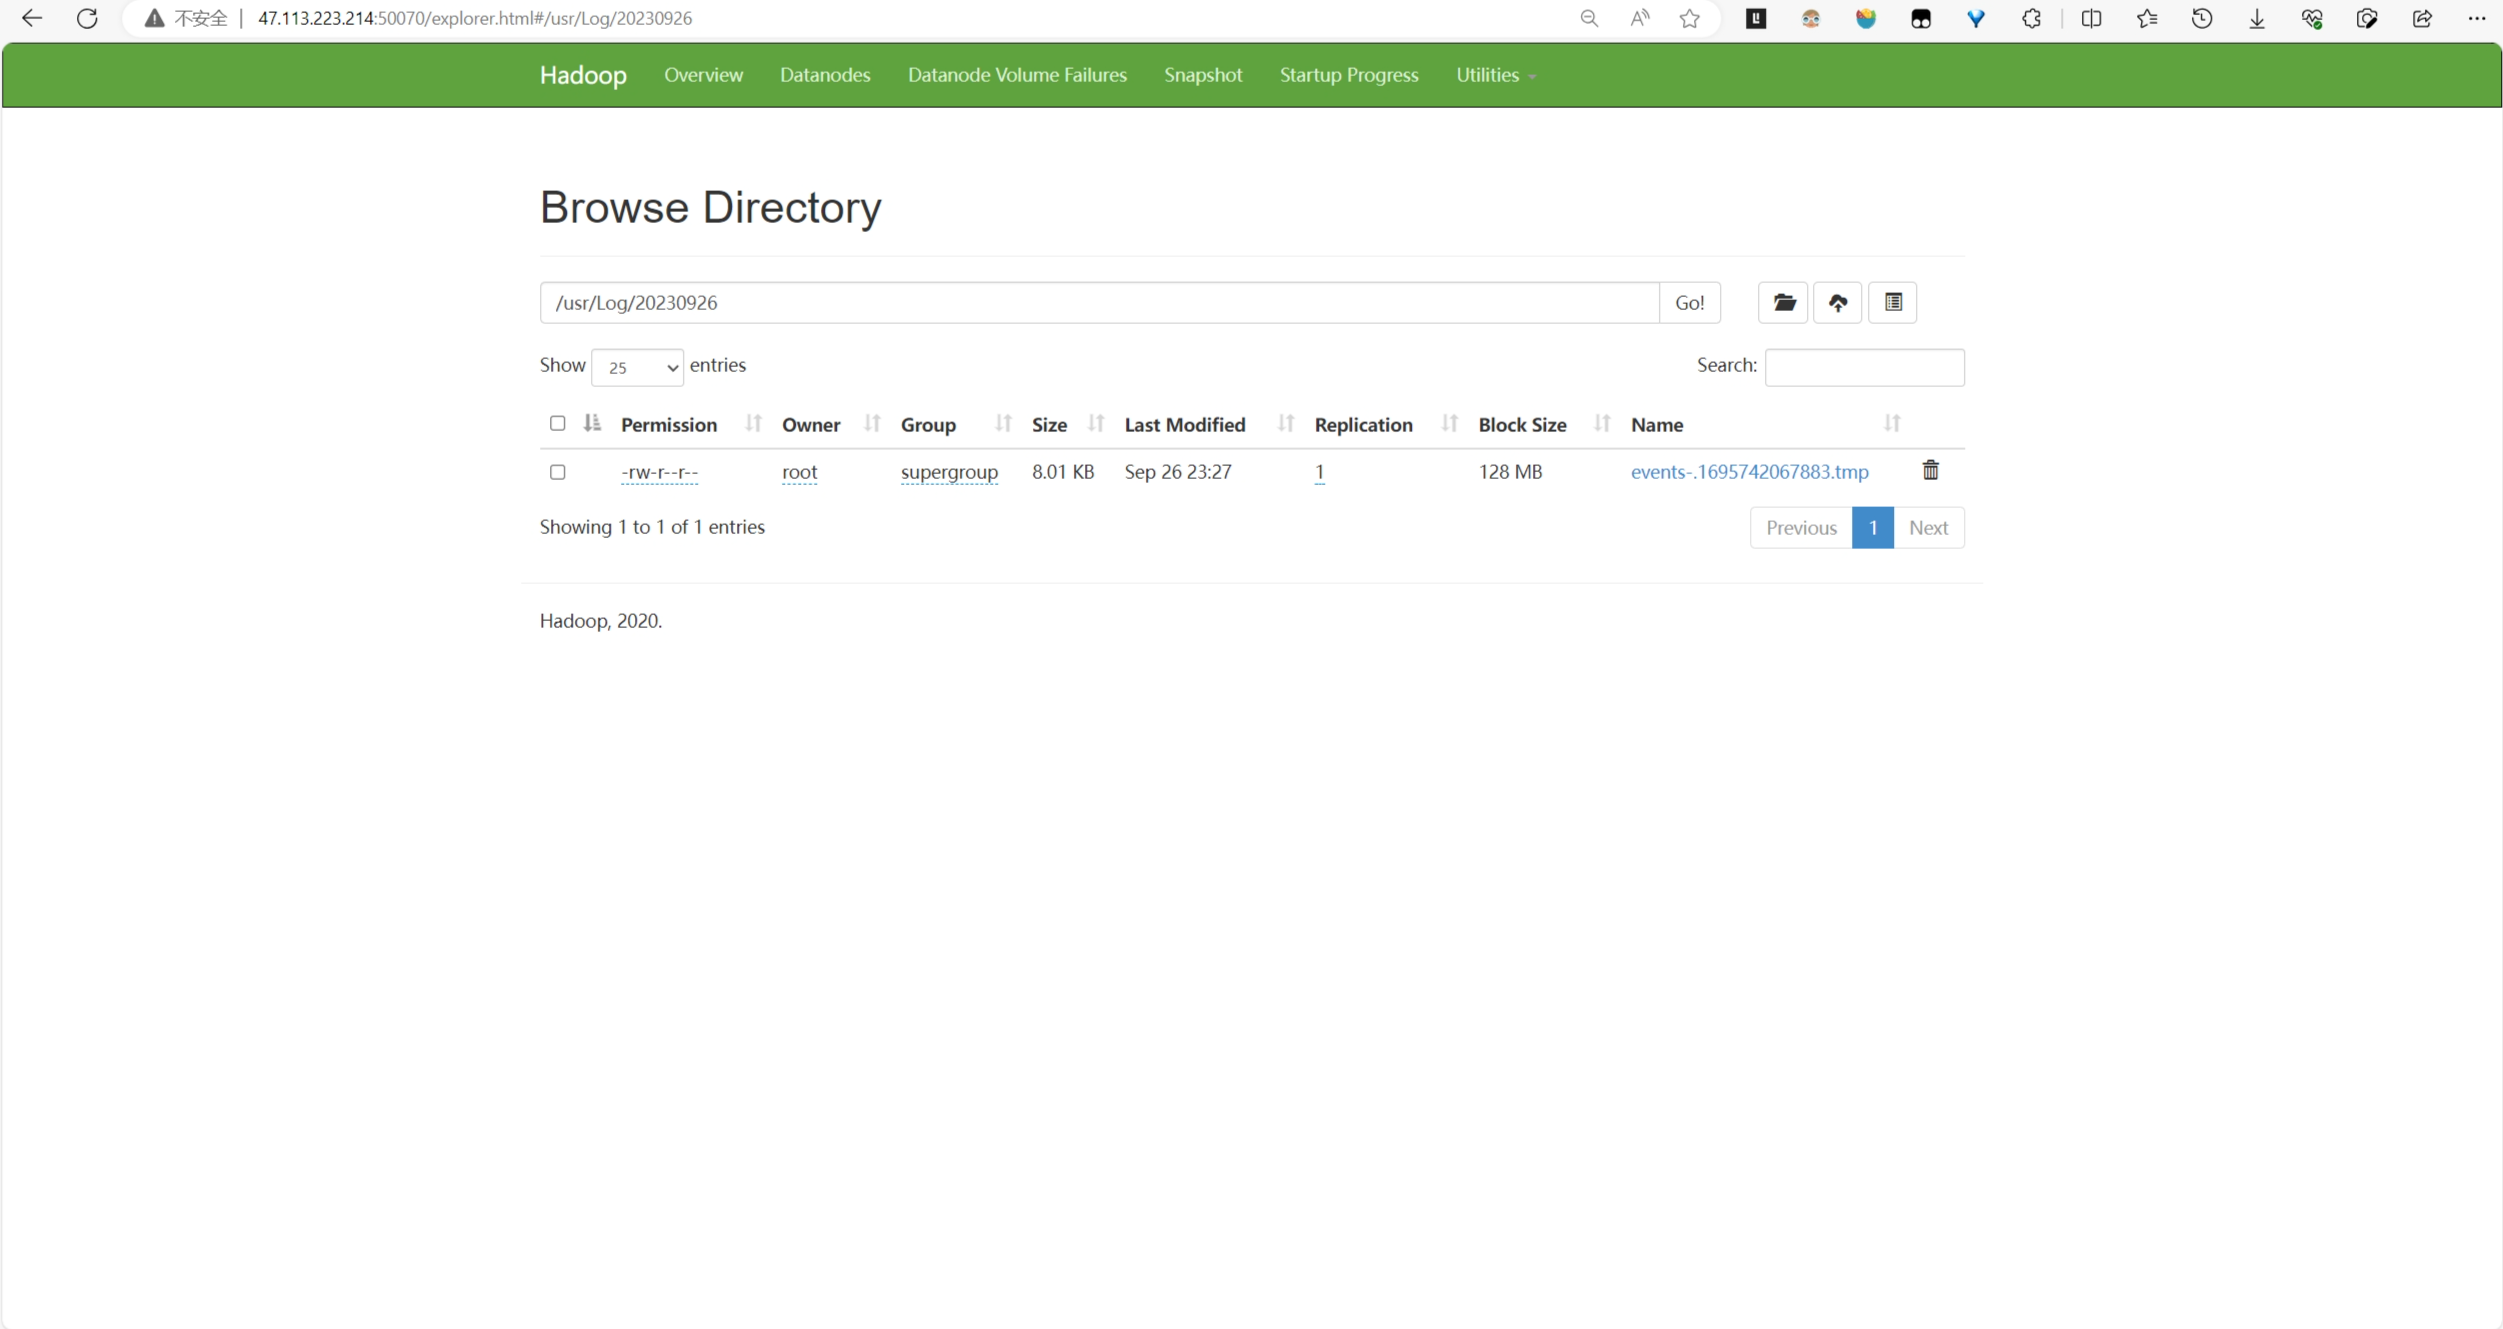
\includegraphics[width=0.7\textwidth]{./pic/17.png}
        \caption{Hadoop}
    \end{figure}
\end{itemize}

\section{困难及克服方法}
在做任务4时发现Flume一直无法把日志文件写入到HDFS里,经过不断查找发现不应该在Flume服务启动前就将.log文件写入目标目录,这样会导致Flume没有监听到。\par
在启动Flume服务后再在目标目录中新建.log文件并写入内容,就可以监听到了。
\end{document}